% ICLR 2027 submission --- MIST
% Official ICLR 2027 conference style and bibliography files ship alongside.
\documentclass[11pt]{article}
\usepackage{iclr2027_conference,times}

\usepackage{graphicx}
\usepackage{amsmath}
\usepackage{amssymb}
\usepackage{booktabs}
\usepackage{multirow}
\usepackage{array}
\usepackage{xcolor}
\usepackage{colortbl}
\usepackage{makecell}
\usepackage{enumitem}
\usepackage{float}
\usepackage{placeins}
\usepackage{tikz}
\usetikzlibrary{arrows.meta,positioning,fit,backgrounds,calc}
\usepackage[most]{tcolorbox}
% LiME-style green callout box for key ideas / findings (bold label + italic body)
\newtcolorbox{keybox}{colback=green!6,colframe=green!45!black,boxrule=0.5pt,arc=2pt,
  left=5pt,right=5pt,top=3pt,bottom=3pt,before skip=6pt,after skip=6pt,fontupper=\small\itshape}
\usepackage[pagebackref,breaklinks,colorlinks]{hyperref}
\usepackage{url}
\usepackage{etoc}   % appendix-only table of contents (Supplementary Material)

% ICLR 2027 submission

\newcommand{\morph}{\textbf{MIST}}
\newcommand{\best}[1]{{\bfseries\boldmath #1}}
\newcommand{\running}{\textcolor{gray}{---}}
\newcommand{\heavytext}[1]{\leavevmode\rlap{\kern0.22pt #1}#1}
\newtheorem{proposition}{Proposition}
\makeatletter
\renewcommand{\@opargbegintheorem}[3]{%
  \trivlist\item[]\noindent{\large\bfseries\heavytext{#1\ #2\ (#3):}}\enspace\normalfont}
\makeatother
\newcommand{\insightbox}[2]{%
  \par\medskip\noindent
  \begingroup
  \setlength{\fboxsep}{7pt}%
  \fcolorbox{blue!55!black}{blue!4}{%
    \parbox{\dimexpr\linewidth-2\fboxsep-2\fboxrule\relax}{%
      \textbf{\textcolor{blue!55!black}{#1}}\quad #2}}%
  \endgroup\par\medskip}
\renewcommand{\arraystretch}{1.05}
\setlength{\textfloatsep}{6pt plus 1pt minus 2pt}
\setlength{\floatsep}{4pt plus 1pt minus 1pt}
\makeatletter
\setlength{\@fptop}{0pt}
\setlength{\@fpbot}{0pt}
\makeatother

\begin{document}

\title{MIST: Integrating Local and Tissue-Wide Context for Gene Expression Prediction from Histology}

\author{Anonymous}
\maketitle

\begin{abstract}
Predicting spatial gene expression from histology requires representations that integrate local morphology with tissue-wide context without depending on arbitrary coordinate conventions. We introduce \morph{}, a spatial transformer that jointly models three complementary sources of context in every layer: local attention over spatial nearest neighbors, global self-attention across all spots, and an attention-pooled slide representation broadcast to each spot. Operating on frozen histology embeddings, \morph{} predicts gene expression for all input spots on a slide in a single forward pass. Spatial coordinates enter only through pairwise distances, making predictions invariant to translations, rotations, and reflections of the coordinate frame when image features are fixed. We evaluate \morph{} on six human organ cohorts from HEST-1k under intra-cohort prediction, pooled multi-organ evaluation, and leave-one-organ-out transfer, using matched features, gene panels, splits, and model-selection procedures across methods. With combined UNI and CONCH features, \morph{} achieves the highest mean Pearson correlation (PCC) across all six cohorts in intra-cohort evaluation, improving over the strongest baseline by $11.6\%$ for 50-gene prediction and $11.4\%$ for 100-gene prediction. It also improves mean correlation in pooled evaluation ($0.599$ versus $0.587$) and transfer to held-out organs ($0.422$ versus $0.398$). In addition to PCC, we also measure MSE and MAE, on which \morph{} likewise outperforms all baselines. Improvements persist across UNI, CONCH, and combined features, while factorial ablations identify local spatial attention as the largest contributor to predictive accuracy. These results support explicit spatial neighborhood modeling within a unified local and tissue-wide representation, while highlighting the remaining difficulty of generalization to unseen organs.
\end{abstract}

\etocdepthtag.toc{mainbody}
\section{Introduction}
Spatial transcriptomics (ST) measures gene expression together with tissue location, enabling the
study of spatial heterogeneity, tissue organization, and cellular interactions
\cite{staahl2016visualization}. Its cost and experimental burden, however, constrain the number and
diversity of specimens that can be profiled. In contrast, H\&E slides are routinely collected and
contain morphological signals associated with tissue composition and molecular state. Predicting
spatial gene expression from these images could therefore extend molecular analysis to specimens
without matched ST measurements.

\begin{figure*}[t]
\centering
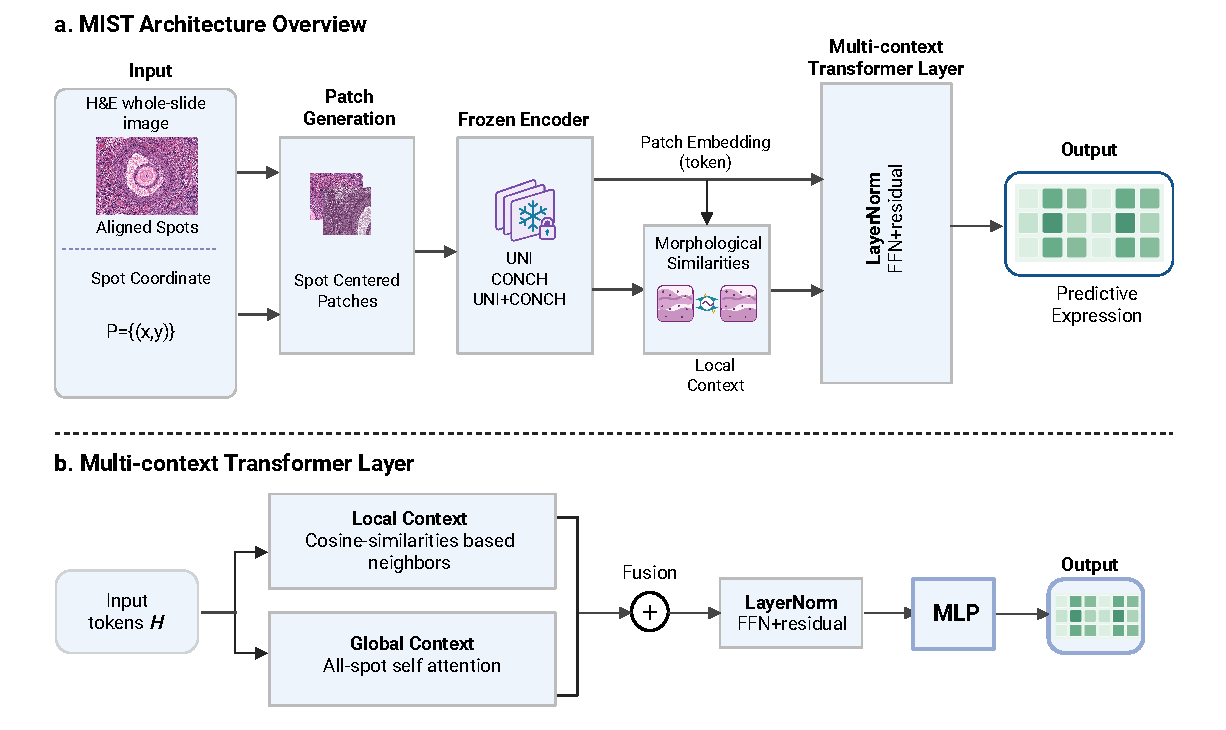
\includegraphics[width=\linewidth]{figures/mist_overview.pdf}
\caption{\textbf{\morph{} overview.} \textbf{(a)}~Frozen UNI, CONCH, or combined features turn
H\&E spot patches into tokens, while coordinate-based $k$NN edges provide local context.
\textbf{(b)}~Each layer combines distance-biased local attention with global self-attention before
the expression head. Pairwise-distance coordinates ensure invariance to translations, rotations,
and reflections.}
\label{fig:arch}
\end{figure*}
\vspace{-6pt}

Morphology and expression interact locally, across the slide, and at the level of slide composition. Existing predictors capture parts of this structure with patch regression, spatial graphs, retrieval, or conditional generation, but absolute coordinates can make predictions depend on an arbitrary scanner frame. We therefore seek a compact predictor that combines multi-scale context while using coordinates only through relative distances.

We introduce \morph{}, a direct spatial transformer that represents each spot as a token and combines spatial $k$NN attention for local context, full self-attention for slide-wide context, and attention pooling for a slide summary. Because spot coordinates enter the model only through pairwise distances, its predictions are invariant to translations, rotations, and reflections when image features are fixed (Fig.~\ref{fig:arch}).

We evaluate matched features, panels, splits, budgets, and nested validation in intra-cohort, pooled cross-organ, and leave-one-organ-out (LOOO) settings. Across six human cohorts, \morph{} reaches mean PCC $0.496$ versus $0.444$ for BLEEP, $0.760$ pooled PCC, and $0.490$ LOOO PCC; local attention is the strongest factorial component. The model has 4.88M parameters and processes 10,000 spots in $64.7$\,ms on an A100.

\begin{table}[t]
\centering
\caption{\textbf{Architectural components across representative H\&E$\to$ST predictors.}
\morph{} is the only model that combines local neighborhood attention, slide-wide global
attention, a slide-level summary token, coordinate invariance, and continuous (distance-expressive)
spatial encoding rather than binary adjacency. $\bullet$~= present, $\circ$~= absent.}
\label{tab:design_comparison}
\small
\setlength{\tabcolsep}{5pt}
\renewcommand{\arraystretch}{1.1}
\begin{tabular}{l ccccc}
\toprule
Method & \makecell{Local\\context} & \makecell{Global\\context} & \makecell{Slide\\token}
       & \makecell{Coord.\\invariant} & \makecell{Cont.\\distance} \\
\midrule
ST-Net~\cite{he2020stnet}       & $\circ$    & $\circ$    & $\circ$    & $\circ$    & $\circ$    \\
HisToGene~\cite{pang2021histogene} & $\circ$  & $\bullet$  & $\circ$    & $\circ$    & $\circ$    \\
Hist2ST~\cite{zeng2022hist2st}  & $\bullet$  & $\bullet$  & $\circ$    & $\circ$    & $\circ$    \\
BLEEP~\cite{xie2023bleep}       & $\circ$    & $\circ$    & $\circ$    & $\circ$    & $\circ$    \\
TRIPLEX~\cite{chung2024triplex} & $\bullet$  & $\bullet$  & $\circ$    & $\circ$    & $\circ$    \\
M2OST~\cite{wang2025m2ost}      & $\bullet$  & $\circ$    & $\circ$    & $\circ$    & $\circ$    \\
STEM~\cite{zhu2025diffusion}    & $\circ$    & $\bullet$  & $\circ$    & $\circ$    & $\circ$    \\
\midrule
\morph{} (ours)                 & $\bullet$  & $\bullet$  & $\bullet$  & $\bullet$  & $\bullet$  \\
\bottomrule
\end{tabular}
\end{table}

\medskip
\noindent We investigate five questions: \textbf{RQ1 (Performance)} accuracy across diverse organs, both per-organ and with a single pooled model; \textbf{RQ2 (Transfer)} generalization to an entirely unseen organ under LOOO; \textbf{RQ3 (Design)} the effect of encoder, context streams, and neighborhood definition; \textbf{RQ4 (Structure)} spatial-domain recovery; and \textbf{RQ5 (Efficiency)} whole-slide inference.

\medskip
\noindent\textbf{Contributions.}
\begin{enumerate}[leftmargin=1.5em,itemsep=1pt,topsep=2pt]
  \item We introduce \morph{}, a multi-scale transformer with local, slide-wide, and slide-summary pathways driven by continuous pairwise-distance features and coordinate-frame invariance.
  \item We quantify the effects of context, distance encoding, and feature choice through matched ablations and transformation tests.
  \item We provide a controlled pooled cross-organ benchmark alongside intra-cohort and held-out-organ evaluation with matched panels, splits, baselines, and model selection.
\end{enumerate}

\iffalse
\begin{figure*}[t]
\centering
\input{figures/trism_overview}
\iffalse
\resizebox{0.98\textwidth}{!}{%
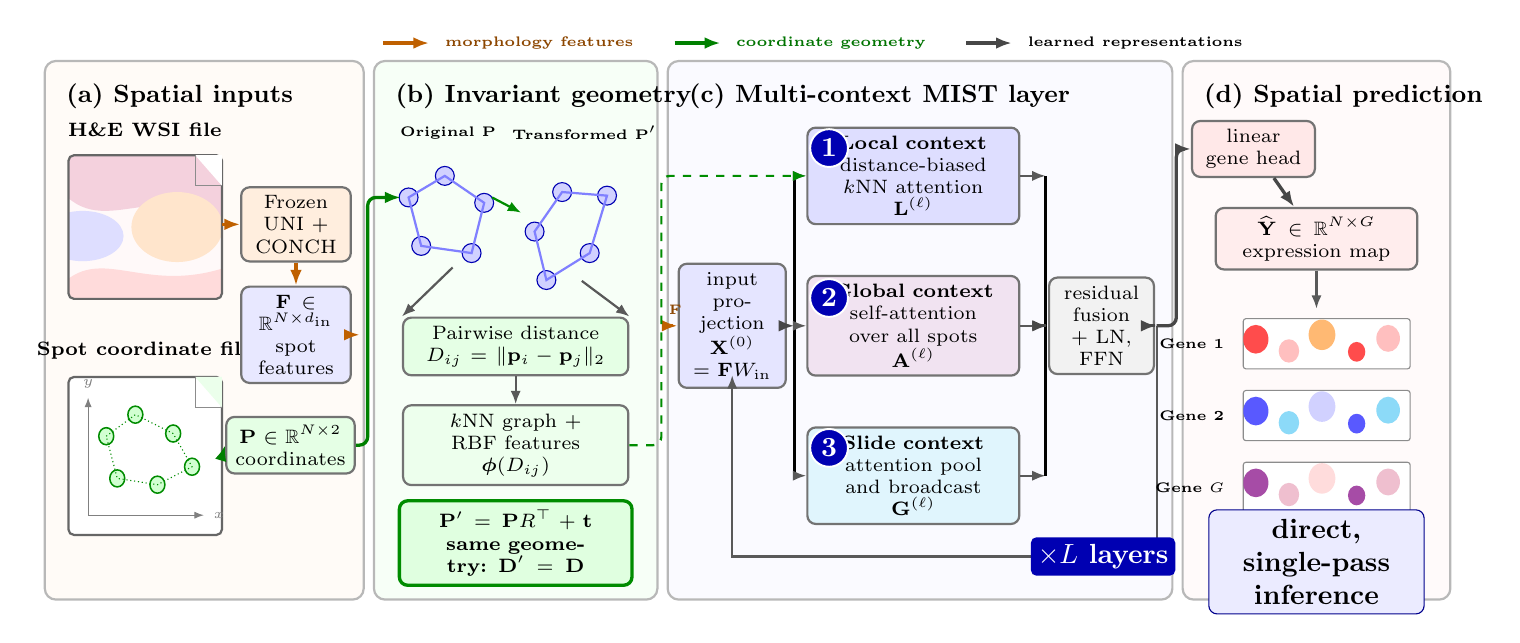
\begin{tikzpicture}[x=1cm,y=1.14cm,font=\scriptsize,
  panel/.style={draw=black!28,thick,rounded corners=4pt,fill=gray!2},
  box/.style={draw=black!55,thick,rounded corners=3pt,align=center,fill=white,
              minimum height=0.62cm,inner sep=3pt},
  flow/.style={-{Latex[length=2mm,width=1.5mm]},very thick,draw=black!72},
  thinflow/.style={-{Latex[length=1.7mm,width=1.3mm]},thick,draw=black!65},
  morphflow/.style={-{Latex[length=2mm,width=1.5mm]},very thick,draw=orange!75!black},
  geomflow/.style={-{Latex[length=2mm,width=1.5mm]},very thick,draw=green!50!black},
  tag/.style={circle,draw=white,line width=0.7pt,fill=blue!70!black,text=white,
              font=\bfseries,inner sep=0pt,minimum size=4.8mm},
  dot/.style={circle,draw=blue!70!black,fill=blue!18,inner sep=0pt,minimum size=2.4mm}]

% Panel backgrounds and headings
\draw[panel,fill=orange!3] (0,0) rectangle (4.05,6.0);
\draw[panel,fill=green!3]  (4.18,0) rectangle (7.78,6.0);
\draw[panel,fill=blue!2]   (7.91,0) rectangle (14.32,6.0);
\draw[panel,fill=red!2]    (14.45,0) rectangle (17.85,6.0);
\node[anchor=north west,font=\small\bfseries] at (0.15,5.86) {(a) Spatial inputs};
\node[anchor=north west,font=\small\bfseries] at (4.33,5.86) {(b) Invariant geometry};
\node[anchor=north west,font=\small\bfseries] at (8.06,5.86) {(c) Multi-context \morph{} layer};
\node[anchor=north west,font=\small\bfseries] at (14.60,5.86) {(d) Spatial prediction};

% Data-flow legend
\draw[morphflow] (4.30,6.20)--(4.88,6.20);
\node[anchor=west,font=\tiny\bfseries,text=orange!55!black] at (4.96,6.20)
  {morphology features};
\draw[geomflow] (8.00,6.20)--(8.58,6.20);
\node[anchor=west,font=\tiny\bfseries,text=green!45!black] at (8.66,6.20)
  {coordinate geometry};
\draw[flow] (11.70,6.20)--(12.28,6.20);
\node[anchor=west,font=\tiny\bfseries] at (12.36,6.20)
  {learned representations};

% (a) Two explicit input files: WSI and spot-coordinate map
\begin{scope}
  \clip[rounded corners=2pt] (0.30,3.35) rectangle (2.25,4.95);
  \fill[pink!10] (0.30,3.35) rectangle (2.25,4.95);
  \fill[purple!18] (0.12,4.65) .. controls (0.72,3.90) and (1.35,4.80) ..
    (2.48,4.12) -- (2.48,5.12) -- (0.12,5.12) -- cycle;
  \fill[red!14] (0.16,3.46) .. controls (0.72,4.02) and (1.28,3.32) ..
    (2.48,3.76) -- (2.48,3.20) -- (0.16,3.20) -- cycle;
  \fill[blue!13] (0.48,4.05) ellipse (0.52 and 0.28);
  \fill[orange!20] (1.68,4.15) ellipse (0.58 and 0.39);
\end{scope}
\draw[black!60,thick,rounded corners=2pt] (0.30,3.35) rectangle (2.25,4.95);
\fill[white] (1.91,4.95)--(2.25,4.61)--(2.25,4.95)--cycle;
\draw[black!45] (1.91,4.95)--(1.91,4.61)--(2.25,4.61);
\node[anchor=south,font=\scriptsize\bfseries] at (1.27,5.05) {H\&E WSI file};

% Coordinate file shown as an independent spatial spot map
\draw[fill=white,draw=black!60,thick,rounded corners=2pt]
  (0.30,0.72) rectangle (2.25,2.48);
\fill[green!8] (1.91,2.48)--(2.25,2.14)--(2.25,2.48)--cycle;
\draw[black!45] (1.91,2.48)--(1.91,2.14)--(2.25,2.14);
\draw[-{Latex[length=1.2mm]},black!50] (0.55,0.94)--(2.02,0.94)
  node[right,font=\tiny] {$x$};
\draw[-{Latex[length=1.2mm]},black!50] (0.55,0.94)--(0.55,2.25)
  node[above,font=\tiny] {$y$};
\foreach \x/\y in {0.78/1.82,1.15/2.06,1.63/1.85,0.92/1.35,1.43/1.28,1.87/1.48}
  \draw[fill=green!18,draw=green!55!black,line width=0.55pt] (\x,\y) circle (0.095);
\draw[green!55!black,densely dotted] (0.78,1.82)--(1.15,2.06)--(1.63,1.85)--
  (1.87,1.48)--(1.43,1.28)--(0.92,1.35)--cycle;
\node[anchor=south,font=\scriptsize\bfseries] at (1.27,2.57) {Spot coordinate file};

\node[box,fill=orange!13,text width=1.18cm] (encoder) at (3.19,4.18)
  {Frozen\\UNI + CONCH};
\node[box,fill=blue!9,text width=1.18cm] (features) at (3.19,2.95)
  {$\mathbf F\in\mathbb R^{N\times d_{\rm in}}$\\spot features};
\node[box,fill=green!10,text width=1.42cm] (coords) at (3.12,1.72)
  {$\mathbf P\in\mathbb R^{N\times2}$\\coordinates};
\draw[morphflow] (2.25,4.18)--(encoder.west);
\draw[morphflow] (encoder)--(features);
\draw[geomflow] (2.25,1.60)--(coords.west);
\draw[morphflow] (features.east)--(4.00,2.95);

% (b) Original and transformed point configurations
\node[font=\tiny\bfseries] at (5.12,5.20) {Original $\mathbf P$};
\node[font=\tiny\bfseries] at (6.85,5.20) {Transformed $\mathbf P'$};
\foreach \x/\y in {4.62/4.48,5.08/4.72,5.58/4.42,4.78/3.94,5.42/3.86}
  \node[dot] at (\x,\y) {};
\draw[blue!50,thick] (4.62,4.48)--(5.08,4.72)--(5.58,4.42)--(5.42,3.86)--(4.78,3.94)--cycle;
\foreach \x/\y in {6.22/4.10,6.57/4.54,7.14/4.50,6.37/3.56,6.92/3.86}
  \node[dot] at (\x,\y) {};
\draw[blue!50,thick] (6.22,4.10)--(6.57,4.54)--(7.14,4.50)--(6.92,3.86)--(6.37,3.56)--cycle;
\draw[thinflow,green!55!black] (5.68,4.48)--(6.05,4.31);
\draw[geomflow,rounded corners=3pt]
  (coords.east)--(4.10,1.72)--(4.10,4.48)--(4.52,4.48);

\node[box,fill=green!10,text width=2.65cm] (distance) at (5.98,2.82)
  {Pairwise distance\\$D_{ij}=\|\mathbf p_i-\mathbf p_j\|_2$};
\node[box,fill=green!7,text width=2.65cm] (rbfnew) at (5.98,1.72)
  {$k$NN graph $+$ RBF features\\$\boldsymbol\phi(D_{ij})$};
\draw[thinflow] (5.18,3.70)--(distance.north west);
\draw[thinflow] (6.82,3.55)--(distance.north east);
\draw[thinflow] (distance)--(rbfnew);
\node[draw=green!55!black,very thick,rounded corners=3pt,fill=green!12,
      align=center,text width=2.72cm,minimum height=0.60cm] at (5.98,0.63)
  {$\mathbf P'=\mathbf P R^\top+\mathbf t$\\\textbf{same geometry:} $\mathbf D'=\mathbf D$};

% (c) Token input and three complementary paths
\node[box,fill=blue!10,text width=1.15cm,minimum height=1.0cm] (tokens) at (8.73,3.05)
  {input projection\\$\mathbf X^{(0)}$\\$=\mathbf F W_{\rm in}$};
\draw[morphflow] (7.98,3.05)--(tokens.west)
  node[midway,above,font=\tiny\bfseries,text=orange!55!black] {$\mathbf F$};
\node[box,fill=blue!13,text width=2.48cm,minimum height=1.08cm] (localnew) at (11.03,4.72)
  {\textbf{Local context}\\distance-biased $k$NN attention\\$\mathbf L^{(\ell)}$};
\node[box,fill=violet!11,text width=2.48cm,minimum height=1.08cm] (globalnew) at (11.03,3.05)
  {\textbf{Global context}\\self-attention over all spots\\$\mathbf A^{(\ell)}$};
\node[box,fill=cyan!12,text width=2.48cm,minimum height=1.08cm] (slidenew) at (11.03,1.38)
  {\textbf{Slide context}\\attention pool and broadcast\\$\mathbf G^{(\ell)}$};
\node[tag] at (9.96,5.03) {1};
\node[tag] at (9.96,3.36) {2};
\node[tag] at (9.96,1.69) {3};
\coordinate (split) at (9.52,3.05);
\draw[flow] (tokens.east)--(split);
\draw[very thick] (9.52,1.38)--(9.52,4.72);
\draw[thinflow] (9.52,4.72)--(localnew.west);
\draw[thinflow] (9.52,3.05)--(globalnew.west);
\draw[thinflow] (9.52,1.38)--(slidenew.west);
\draw[thinflow,green!55!black,dashed,rounded corners=3pt]
  (rbfnew.east)--(7.83,1.72)--(7.83,4.72)--(localnew.west);

\node[box,fill=gray!10,text width=1.12cm,minimum height=1.18cm] (fusionnew) at (13.42,3.05)
  {residual\\fusion\\$+$ LN, FFN};
\coordinate (join) at (12.71,3.05);
\draw[thinflow] (localnew.east)--(12.71,4.72);
\draw[thinflow] (globalnew.east)--(12.71,3.05);
\draw[thinflow] (slidenew.east)--(12.71,1.38);
\draw[very thick] (12.71,4.72)--(12.71,1.38);
\draw[flow] (join)--(fusionnew.west);
\draw[flow] (fusionnew.east) -- (14.12,3.05);
\draw[thinflow] (14.12,3.05) |- (13.42,0.48) -| (8.73,2.50);
\node[fill=blue!70!black,text=white,rounded corners=2pt,font=\bfseries,
      inner sep=2.5pt] at (13.44,0.48) {$\times L$ layers};

% (d) Output head and stylized spatial gene maps
\node[box,fill=red!9,text width=1.35cm] (head) at (15.35,5.02)
  {linear\\gene head};
\draw[flow,rounded corners=3pt] (14.12,3.05)--(14.37,3.05)--(14.37,5.02)--(head.west);
\node[box,fill=red!7,text width=2.35cm,minimum height=0.72cm] (ymap) at (16.15,4.02)
  {$\widehat{\mathbf Y}\in\mathbb R^{N\times G}$\\expression map};
\draw[flow] (head)--(ymap);
\draw[thinflow] (ymap.south)--(16.15,3.24);

\foreach \yy/\lab/\ca/\cb/\cc in {2.85/Gene 1/red!70/red!25/orange!55,
                                     2.05/Gene 2/blue!65/cyan!45/blue!18,
                                     1.25/Gene $G$/violet!70/purple!25/pink!55}{
  \node[anchor=east,font=\tiny\bfseries] at (15.10,\yy) {\lab};
  \draw[rounded corners=1pt,fill=white,draw=black!45] (15.22,\yy-0.28) rectangle (17.34,\yy+0.28);
  \fill[\ca] (15.38,\yy+0.05) circle (0.16);
  \fill[\cb] (15.80,\yy-0.08) circle (0.13);
  \fill[\cc] (16.22,\yy+0.10) circle (0.17);
  \fill[\ca] (16.66,\yy-0.09) circle (0.11);
  \fill[\cb] (17.06,\yy+0.06) circle (0.15);
}
\node[draw=blue!55!black,rounded corners=3pt,fill=blue!8,font=\bfseries,
      align=center,text width=2.50cm,minimum height=0.58cm] at (16.15,0.42)
  {direct, single-pass inference};
\end{tikzpicture}
}
\fi
\caption{\textbf{\morph{} overview.}
\textbf{(a)} The model receives two aligned files: an H\&E whole slide image and a file containing
the $x,y$ coordinate of each measured spot. Frozen pathology encoders represent spot morphology,
while the coordinate file provides tissue geometry. Orange arrows trace morphology features, green
arrows trace coordinate geometry, and black arrows trace learned representations. \textbf{(b)} Coordinates enter the model only through pairwise
distances, which define a shared $k$NN graph and radial basis features and are unchanged by
translations, rotations, and reflections. \textbf{(c)} Every layer combines distance-biased local
attention, global self-attention, and an attention-pooled slide representation through residual
fusion. \textbf{(d)} After $L$ layers, a linear head directly predicts a spatial expression map for
all genes in one pass.}
\label{fig:arch}
\end{figure*}
\fi

\section{Related Work}
\noindent\textbf{H\&E$\to$ST prediction.}\quad Prior models span patch-level regression
(ST-Net~\cite{he2020stnet}), graph spatial context (Hist2ST~\cite{zeng2022hist2st}), cross-modal
retrieval (BLEEP~\cite{xie2023bleep}), and conditional generation (STEM~\cite{zhu2025diffusion}).
Because they differ in features, gene panels, splits, and selection, published scores conflate data
choices with architecture; we therefore compare under a matched protocol. \morph{} is a deterministic
point predictor and does not model the full conditional expression distribution.

\medskip
\noindent\textbf{Geometry and generalization.}\quad Absolute position encodings can change when an
equivalent tissue layout is translated, rotated, or reflected; geometric networks instead build
interactions from relative quantities~\cite{satorras2021egnn}. \morph{} conditions its spatial
pathway only on pairwise Euclidean distances, invariant to such frame changes for fixed histology
features. For generalization we separate pooled cross-validation (organs seen, samples held out) from
LOOO (an entire organ withheld) to isolate anatomical transfer on HEST-1k~\cite{jaume2024hest}. An
extended discussion and positioning of \morph{} are in Appendix~\ref{app:related}.

\section{Method}

MIST maps frozen spot-level histology features and measured spot coordinates to a spatial gene
expression map. Its method has three stages: coordinate-invariant distance encoding, a shared
multi-context layer, and supervised prediction with a correlation-aware objective.

\subsection{Problem Setup}
For a slide with $N$ spots, let
$\mathbf{F}=[\mathbf{f}_1,\ldots,\mathbf{f}_N]^\top\in\mathbb{R}^{N\times d_{\mathrm{in}}}$
denote frozen pathology features and
$\mathbf{P}=[\mathbf{p}_1,\ldots,\mathbf{p}_N]^\top\in\mathbb{R}^{N\times2}$ the corresponding
spot coordinates. The target
$\mathbf{Y}\in\mathbb{R}^{N\times G}$ contains log-normalized expression for $G$ genes. We learn
$f_\theta:(\mathbf{F},\mathbf{P})\mapsto\hat{\mathbf{Y}}$ and process each slide independently;
the model therefore supports a variable number of spots and does not require expression measurements at
test time. In the feature-matched main comparisons, $\mathbf{f}_i$ concatenates frozen UNI
\cite{chen2024uni} and CONCH \cite{lu2024conch} embeddings ($d_{\mathrm{in}}=1536$).

\medskip
\subsection{Coordinate-Invariant Distance Encoding}
We first compute the pairwise Euclidean distance matrix
$D_{ij}=\lVert\mathbf{p}_i-\mathbf{p}_j\rVert_2$. For each spot $i$, we retain the indices
$\mathcal{N}(i)$ and distances of its $k$ nearest neighbors, excluding the spot itself. Distances
are expanded into $M$ radial-basis features,
\begin{equation}
\boldsymbol{\phi}(D_{ij})=
\left[\exp\!\left(-\gamma_m D_{ij}^{2}\right)\right]_{m=1}^{M},
\end{equation}
where the fixed bandwidth parameters $\gamma_m$ are logarithmically spaced. These features influence
attention weights but are never added to the spot embeddings as absolute positions.

\par\medskip\noindent\refstepcounter{proposition}\textbf{Proposition \theproposition\ (Coordinate frame invariance):}\label{prop:coordinate_invariance}\par
Let $R\in\mathbb{R}^{2\times2}$ be orthogonal, let $\mathbf{t}\in\mathbb{R}^{2}$, and define
$\mathbf{P}'=\mathbf{P}R^\top+\mathbf{1}\mathbf{t}^\top$. For fixed histology features
$\mathbf{F}$, the prediction is unchanged:
\begin{equation}
f_\theta(\mathbf{F},\mathbf{P}')=f_\theta(\mathbf{F},\mathbf{P}).
\end{equation}
Thus, the spatial pathway is invariant to translations, rotations, and reflections of the coordinate
frame in exact arithmetic.
The guarantee concerns a change of coordinate frame with fixed histology features; it does not claim
that the frozen image encoder is invariant to transformations of the histology image. The proof is in
Appendix~\ref{app:formal_guarantees}.
The RBF bias is available to weight neighbors by distance, but at native HEST pixel scale the
neighbor distances ($\sim\!10^{3}$) saturate $\exp(-\gamma D^{2})$ toward zero for all bandwidths, so
in the reported configuration the bias contributes negligibly and the local pathway reduces to
attention over the spatial $k$NN neighborhood. The distinguishing property of \morph{} is therefore
this \emph{spatial locality} (each spot aggregates from its geometric neighbors rather than from
arbitrary or random spots), which our ablation isolates directly (spatial $k$NN vs.\ random
neighbors, \S\ref{sec:design}). The invariance guarantee above holds regardless, since it depends
only on distances being rotation-invariant.

\medskip
\subsection{Multi-Context MIST Layer}
\insightbox{Core Idea.}{At every layer, each spot receives three messages in parallel: one from its
nearby spots, one from all spots, and one from a pooled summary of the slide. The model adds these
messages to the current spot representation and refines the result with a feed-forward network.
Only the nearby-spot message uses coordinates, and it uses pairwise distances rather than absolute
positions.}

The input features are projected to hidden width $d$,
$\mathbf{X}^{(0)}=\mathbf{F}W_{\mathrm{in}}+\mathbf{b}_{\mathrm{in}}$. The same neighbor graph and
radial-basis features are reused in all $L$ transformer layers. At layer $\ell$, a pre-normalized
representation $\mathbf{H}=\operatorname{LN}(\mathbf{X}^{(\ell)})$ is passed through three context
pathways.

\subsubsection{Local distance-biased attention}
Each spot attends to its $k$ neighbors with a
learned, distance-dependent bias for each attention head. For head $h$, the attention weights are
\begin{equation}
\alpha_{ij}^{h}=\operatorname{softmax}_{j\in\mathcal{N}(i)}\!\left(
\frac{(\mathbf{q}_i^{h})^\top\mathbf{k}_j^{h}}{\sqrt{d_h}}
+b_h\!\left(\boldsymbol{\phi}(D_{ij})\right)\right),
\end{equation}
where $d_h=d/H$ for $H$ heads. The local output is the concatenation of the weighted value sums,
followed by a learned output projection. Morphological similarity is captured by the query--key
term, while spatial distance contributes through the learned radial-basis bias.

\subsubsection{Global self-attention}
In parallel, standard multi-head self-attention
\cite{vaswani2017attention} allows every spot to attend to all $N$ spots. This pathway captures
long-range dependencies that may not be connected in the local graph. It uses morphology features
only and is permutation-equivariant with respect to spot order.

\subsubsection{Attention-pooled slide context}
A learned scalar scoring function produces
$a_i=\operatorname{softmax}_{i}(s(\mathbf{h}_i))$. The slide representation is
\begin{equation}
\mathbf{g}=W_g\left(\sum_{i=1}^{N}a_i\mathbf{h}_i\right)+\mathbf{b}_g,
\end{equation}
and is broadcast to every spot. Unlike a learned class token, this representation is computed
directly from the slide's spot features and summarizes its morphological composition.

For the complete model, the local ($\mathbf{L}$), global ($\mathbf{G}$), and broadcast slide
($\mathbf{S}$) representations are summed and added to the residual stream. A second
pre-normalization residual update applies a two-layer feed-forward network with expansion factor four
and GELU activation:
\begin{align}
\widetilde{\mathbf{X}}^{(\ell)}
  &=\mathbf{X}^{(\ell)}+\mathbf{L}^{(\ell)}+\mathbf{G}^{(\ell)}+\mathbf{S}^{(\ell)},\\
\mathbf{X}^{(\ell+1)}
  &=\widetilde{\mathbf{X}}^{(\ell)}+
    \operatorname{FFN}\!\left(\operatorname{LN}(\widetilde{\mathbf{X}}^{(\ell)})\right).
\end{align}
After $L$ layers, layer normalization and a linear head map each spot representation to its $G$
predicted gene values. The model produces the complete slide prediction in one forward pass.

\par\medskip\noindent\refstepcounter{proposition}\textbf{Proposition \theproposition\ (Permutation equivariance):}\label{prop:permutation_equivariance}\par
Let $Q\in\{0,1\}^{N\times N}$ be a permutation matrix. If the $k$NN construction handles distance
ties equivariantly, then
\begin{equation}
f_\theta(Q\mathbf{F},Q\mathbf{P})=Qf_\theta(\mathbf{F},\mathbf{P}).
\end{equation}
Therefore, reordering the input spots only reorders their predicted expression profiles.
Appendix~\ref{app:formal_guarantees} provides the proof. Our numerical checks evaluate both
Propositions~\ref{prop:coordinate_invariance} and~\ref{prop:permutation_equivariance} under finite
precision.

\medskip
\subsection{Training Objective and Ablations}
\label{sec:loss}
For a slide with measured expression $\mathbf{Y}$, we optimize mean squared error together with a
gene-wise Pearson-correlation term:
\begin{equation}
\mathcal{L}=\mathrm{MSE}(\hat{\mathbf{Y}},\mathbf{Y})
+ \lambda\left(1-\frac{1}{|\mathcal{V}|}\sum_{g\in\mathcal{V}}\rho_g\right),
\end{equation}
where $\rho_g$ is the Pearson correlation between predicted and measured expression across the $N$
spots, $\mathcal{V}$ is the set of genes with nonzero target variance on that slide, and
$\lambda=0.5$. MSE constrains the scale of the predictions, while the correlation term encourages
the model to reproduce spot-to-spot expression patterns; Appendix~\ref{app:lossdata} ablates this
correlation term.

The main model enables all three context pathways. Our factorial ablation independently toggles the
local (L), global (G), and slide-level (S) pathways, avoiding conclusions tied to a particular order
of architectural additions.






\section{Experimental Setup}
\label{sec:setup}
We evaluate on \textbf{HEST-1k} \cite{jaume2024hest} with frozen UNI+CONCH patch features
(Appendix~\ref{app:encoder} ablates each encoder in isolation) and
$\log(1+x)$ targets; unless stated otherwise the target is the 50-gene HEST HVG panel. To test
robustness to how the target genes are chosen, we use three 50-gene \emph{selection strategies}:
\textbf{HVG}, the highest-variance genes; \textbf{DEG}, differentially expressed genes selected by a
Wilcoxon test across Leiden clusters; and \textbf{HMHVG}, a mean-and-variability criterion applied
after variance filtering (Table~\ref{tab:panel_strategy}). Cross-organ
experiments use the six retained cohorts of Appendix~\ref{app:cohort_stats} (HCC, LYMPH\_IDC, and
READ excluded). We study three regimes: \emph{intra-cohort} (a model per organ), \emph{pooled}
(train across organs, hold out slide-level samples; organ identity is not a model input), and
\emph{LOOO} (train on all-but-one organ, test the held-out organ).
\textbf{Evaluation metrics.} Our primary metric is the \textbf{Pearson correlation coefficient (PCC)}
computed per gene between predicted and measured expression and averaged over genes (genes with zero
target variance are excluded). We also report the \textbf{mean squared error (MSE)} and
\textbf{mean absolute error (MAE)} to capture prediction scale, and, for the spatial-domain-recovery
analysis, the \textbf{Adjusted Rand Index (ARI)} and \textbf{Normalized Mutual Information (NMI)}
between domains clustered from predicted versus measured expression; efficiency is measured by
inference latency and peak GPU memory. All metrics are averaged over outer folds and three seeds, with
checkpoints chosen on inner validation and evaluated once on the outer fold. Baselines ST-Net \cite{he2020stnet}, Hist2ST \cite{zeng2022hist2st}, BLEEP
\cite{xie2023bleep}, and STEM \cite{zhu2025diffusion} use matched features, panels, splits, budgets,
and selection. \morph{} has 4.88M parameters (four layers, width 256, eight neighbors). Full dataset,
gene-panel, protocol, and hyperparameter details are in Appendix~\ref{app:extended_setup}.

\section{Results}
\label{sec:results}

\medskip
\subsection{RQ1: Predictive performance across diverse organs}
\label{sec:rq1}
We begin by asking whether \morph{} predicts spatial expression accurately on organs it has
\emph{seen} during training. To answer this, we measure accuracy in two complementary ways under
matched features, panels, and splits: a separate model trained \emph{per cohort} (intra-cohort), and a
\emph{single} model trained jointly across all organs (pooled).

Starting with the intra-cohort setting, we stress-test accuracy along two axes of the target panel and
report both. \emph{First}, across the three 50-gene \emph{selection strategies}
(Table~\ref{tab:panel_strategy}), \morph{} attains the best mean PCC under every strategy: $0.496$
(HVG), $0.615$ (DEG), and $0.650$ (HMHVG), each ahead of the strongest baseline (BLEEP at $0.444$,
$0.559$, and $0.587$, respectively). \emph{Second}, across \emph{panel sizes} (Table~\ref{tab:main}),
this lead persists at every size, as \morph{} tops the average at PCC@10 ($0.600$), PCC@50 ($0.496$),
and PCC@100 ($0.559$). Focusing on the default PCC@50 panel, the gain over BLEEP is $11.6\%$, and
\morph{} wins all six cohorts, with the margin widest on kidney and prostate ($+0.072$, $+0.064$) and
narrowest on lung ($+0.024$); at the smallest 10-gene panel, correlations rise across all methods
because the retained genes are the most variable, and hence the most predictable. Crucially, these
gains are not an artifact of the correlation metric: as Table~\ref{tab:error_strategy} reports,
\morph{} also achieves the lowest error under every strategy and size (for example, at PCC@50 its
MSE is $1.233$ and MAE $0.794$, versus $1.318$ and $0.819$ for BLEEP).
These intra-cohort gains are statistically significant, not noise: across the six cohorts and three
seeds ($n{=}18$ paired runs), \morph{}'s mean PCC@50 exceeds BLEEP's by $0.051$
(95\% bootstrap CI $[0.041,0.062]$; Wilcoxon signed-rank $p{=}7.6\times10^{-6}$, paired $t$-test
$p{=}4.7\times10^{-8}$), and at the finer per-gene level \morph{} outperforms BLEEP on $87\%$ of genes
($n{=}300$; Wilcoxon $p<10^{-30}$). Appendix~\ref{app:significance} reports the full paired tests for
all regimes, including the significant LOOO gain and the marginal pooled one.

% Keep all three gene-selection strategies in one indivisible float.
\begin{table*}[!t]
\centering
\caption{\textbf{Intra-cohort PCC across 50-gene selection strategies.} Mean$_{\text{std}}$ over three seeds.}
\label{tab:panel_strategy}
\setlength{\tabcolsep}{3pt}
\renewcommand{\arraystretch}{0.85}
\resizebox{0.68\linewidth}{!}{%
\begin{tabular}{llccccc}
\toprule
Panel & Cohort & ST-Net & Hist2ST
      & BLEEP & STEM & \morph{} (Ours) \\
\midrule
\multirow{7}{*}{\textbf{HVG}} & IDC & $0.551{\pm}0.01$ & $0.305{\pm}0.11$ & $0.519{\pm}0.00$ & $0.434{\pm}0.00$ & \best{$0.581{\pm}0.01$} \\
 & CCRCC & $0.163{\pm}0.02$ & $0.180{\pm}0.03$ & $0.175{\pm}0.02$ & $0.118{\pm}0.01$ & \best{$0.252{\pm}0.01$} \\
 & LUNG & $0.521{\pm}0.01$ & $0.430{\pm}0.05$ & $0.565{\pm}0.01$ & $0.407{\pm}0.00$ & \best{$0.589{\pm}0.01$} \\
 & PAAD & $0.366{\pm}0.03$ & $0.248{\pm}0.04$ & $0.412{\pm}0.03$ & $0.233{\pm}0.02$ & \best{$0.437{\pm}0.03$} \\
 & PRAD & $0.287{\pm}0.02$ & $0.323{\pm}0.01$ & $0.346{\pm}0.01$ & $0.207{\pm}0.02$ & \best{$0.410{\pm}0.01$} \\
 & SKCM & $0.661{\pm}0.01$ & $0.523{\pm}0.00$ & $0.650{\pm}0.00$ & $0.461{\pm}0.02$ & \best{$0.707{\pm}0.01$} \\
\cmidrule(lr){2-7}
 & \textbf{Average} & $0.425$ & $0.335$ & $0.444$ & $0.310$ & \best{$0.496$} \\
\midrule
\multirow{7}{*}{\textbf{DEG}} & IDC & $0.697{\pm}0.01$ & $0.549{\pm}0.07$ & $0.731{\pm}0.01$ & $0.684{\pm}0.02$ & \best{$0.774{\pm}0.01$} \\
 & CCRCC & $0.312{\pm}0.01$ & $0.335{\pm}0.01$ & $0.304{\pm}0.00$ & $0.253{\pm}0.01$ & \best{$0.402{\pm}0.01$} \\
 & LUNG & $0.566{\pm}0.01$ & $0.518{\pm}0.01$ & $0.621{\pm}0.01$ & $0.440{\pm}0.01$ & \best{$0.662{\pm}0.00$} \\
 & PAAD & $0.425{\pm}0.03$ & $0.352{\pm}0.01$ & $0.487{\pm}0.03$ & $0.306{\pm}0.04$ & \best{$0.518{\pm}0.03$} \\
 & PRAD & $0.413{\pm}0.00$ & $0.437{\pm}0.01$ & $0.466{\pm}0.00$ & $0.355{\pm}0.03$ & \best{$0.539{\pm}0.01$} \\
 & SKCM & $0.752{\pm}0.01$ & $0.656{\pm}0.00$ & $0.746{\pm}0.03$ & $0.617{\pm}0.02$ & \best{$0.794{\pm}0.00$} \\
\cmidrule(lr){2-7}
 & \textbf{Average} & $0.528$ & $0.475$ & $0.559$ & $0.443$ & \best{$0.615$} \\
\midrule
\multirow{7}{*}{\textbf{HMHVG}} & IDC & $0.724{\pm}0.01$ & $0.633{\pm}0.08$ & $0.739{\pm}0.02$ & $0.687{\pm}0.01$ & \best{$0.774{\pm}0.01$} \\
 & CCRCC & $0.339{\pm}0.01$ & $0.387{\pm}0.01$ & $0.349{\pm}0.01$ & $0.290{\pm}0.01$ & \best{$0.454{\pm}0.02$} \\
 & LUNG & $0.568{\pm}0.00$ & $0.598{\pm}0.00$ & $0.661{\pm}0.00$ & $0.517{\pm}0.01$ & \best{$0.693{\pm}0.00$} \\
 & PAAD & $0.441{\pm}0.03$ & $0.341{\pm}0.04$ & $0.493{\pm}0.02$ & $0.305{\pm}0.03$ & \best{$0.524{\pm}0.02$} \\
 & PRAD & $0.452{\pm}0.00$ & $0.477{\pm}0.01$ & $0.432{\pm}0.04$ & $0.337{\pm}0.02$ & \best{$0.555{\pm}0.02$} \\
 & SKCM & $0.824{\pm}0.03$ & $0.710{\pm}0.14$ & $0.849{\pm}0.02$ & $0.731{\pm}0.06$ & \best{$0.901{\pm}0.00$} \\
\cmidrule(lr){2-7}
 & \textbf{Average} & $0.558$ & $0.524$ & $0.587$ & $0.478$ & \best{$0.650$} \\
\bottomrule
\end{tabular}%
}

\medskip
\centering
\caption{\textbf{Intra-cohort PCC across gene-panel sizes.} Mean$_{\text{std}}$ over three seeds; each panel reports its average.}
\label{tab:main}
\label{tab:main_g10}
\label{tab:main_g100}
\setlength{\tabcolsep}{3pt}
\renewcommand{\arraystretch}{0.85}
\resizebox{0.68\linewidth}{!}{%
\begin{tabular}{llccccc}
\toprule
Metric & Cohort & ST-Net & Hist2ST
       & BLEEP & STEM & \morph{} (Ours) \\
\midrule
\multirow{7}{*}{\textbf{PCC@10}} & IDC & $0.666{\pm}0.01$ & $0.636{\pm}0.01$ & $0.635{\pm}0.02$ & $0.591{\pm}0.02$ & \best{$0.708{\pm}0.00$} \\
 & CCRCC & $0.231{\pm}0.01$ & $0.273{\pm}0.02$ & $0.231{\pm}0.02$ & $0.170{\pm}0.00$ & \best{$0.322{\pm}0.01$} \\
 & LUNG & $0.702{\pm}0.01$ & $0.519{\pm}0.02$ & $0.735{\pm}0.00$ & $0.616{\pm}0.01$ & \best{$0.759{\pm}0.00$} \\
 & PAAD & $0.511{\pm}0.04$ & $0.377{\pm}0.07$ & \best{$0.536{\pm}0.03$} & $0.393{\pm}0.04$ & $0.519{\pm}0.05$ \\
 & PRAD & $0.442{\pm}0.03$ & $0.459{\pm}0.02$ & $0.434{\pm}0.03$ & $0.325{\pm}0.03$ & \best{$0.524{\pm}0.02$} \\
 & SKCM & $0.728{\pm}0.00$ & $0.471{\pm}0.04$ & $0.697{\pm}0.01$ & $0.598{\pm}0.01$ & \best{$0.769{\pm}0.01$} \\
\cmidrule(lr){2-7}
 & \textbf{Average} & $0.547$ & $0.456$ & $0.545$ & $0.449$ & \best{$0.600$} \\
\midrule
\multirow{7}{*}{\textbf{PCC@50}} & IDC      & $0.551{\pm}0.01$ & $0.309{\pm}0.07$ & $0.519{\pm}0.00$ & $0.439{\pm}0.01$ & \best{$0.581{\pm}0.01$} \\
 & CCRCC    & $0.163{\pm}0.02$ & $0.184{\pm}0.02$ & $0.175{\pm}0.02$ & $0.123{\pm}0.00$ & \best{$0.252{\pm}0.01$} \\
 & LUNG       & $0.518{\pm}0.01$ & $0.470{\pm}0.01$ & $0.562{\pm}0.01$ & $0.423{\pm}0.03$ & \best{$0.589{\pm}0.01$} \\
 & PAAD       & $0.366{\pm}0.03$ & $0.248{\pm}0.04$ & $0.412{\pm}0.03$ & $0.233{\pm}0.02$ & \best{$0.437{\pm}0.03$} \\
 & PRAD   & $0.294{\pm}0.02$ & $0.333{\pm}0.02$ & $0.348{\pm}0.01$ & $0.207{\pm}0.02$ & \best{$0.410{\pm}0.01$} \\
 & SKCM       & $0.665{\pm}0.01$ & $0.522{\pm}0.03$ & $0.645{\pm}0.01$ & $0.491{\pm}0.04$ & \best{$0.707{\pm}0.01$} \\
\cmidrule(lr){2-7}
 & \textbf{Average} & $0.425$ & $0.335$ & $0.444$ & $0.310$ & \best{$0.496$} \\
\midrule
\multirow{7}{*}{\textbf{PCC@100}} & IDC & $0.611{\pm}0.01$ & $0.473{\pm}0.07$ & $0.632{\pm}0.01$ & $0.565{\pm}0.01$ & \best{$0.682{\pm}0.01$} \\
 & CCRCC & $0.221{\pm}0.01$ & $0.274{\pm}0.03$ & $0.247{\pm}0.02$ & $0.192{\pm}0.00$$^\dag$ & \best{$0.328{\pm}0.02$} \\
 & LUNG & $0.595{\pm}0.00$ & $0.434{\pm}0.03$ & $0.659{\pm}0.01$ & $0.498{\pm}0.03$ & \best{$0.688{\pm}0.00$} \\
 & PAAD & $0.355{\pm}0.04$ & $0.222{\pm}0.04$ & $0.399{\pm}0.04$ & $0.236{\pm}0.02$ & \best{$0.435{\pm}0.03$} \\
 & PRAD & $0.327{\pm}0.01$ & $0.341{\pm}0.03$ & $0.377{\pm}0.02$ & $0.240{\pm}0.03$ & \best{$0.450{\pm}0.00$} \\
 & SKCM & $0.696{\pm}0.01$ & $0.446{\pm}0.12$ & $0.696{\pm}0.01$ & $0.602{\pm}0.02$ & \best{$0.771{\pm}0.01$} \\
\cmidrule(lr){2-7}
 & \textbf{Average} & $0.468$ & $0.365$ & $0.502$ & $0.389$ & \best{$0.559$} \\
\bottomrule
\end{tabular}%
}
\end{table*}

\begin{table}[H]
\centering
\caption{\textbf{Error metrics across gene-selection strategies and panel sizes on HEST-1k.}
Mean over three seeds, averaged over the same six cohorts as Tables~\ref{tab:panel_strategy}
and~\ref{tab:main} (IDC, CCRCC, LUNG, PAAD, PRAD, SKCM); lower values are better and the best
result in each row is in \best{bold}. Models, features, splits, and training budget are matched.}
\label{tab:error_strategy}
\setlength{\tabcolsep}{5pt}
\renewcommand{\arraystretch}{1.12}
\resizebox{\linewidth}{!}{%
\begin{tabular}{ll>{\columncolor{blue!5}}c>{\columncolor{blue!5}}c>{\columncolor{blue!5}}c>{\columncolor{blue!5}}c>{\columncolor{blue!5}}c>{\columncolor{orange!7}}c>{\columncolor{orange!7}}c>{\columncolor{orange!7}}c>{\columncolor{orange!7}}c>{\columncolor{orange!7}}c}
\toprule
& & \multicolumn{5}{c}{\cellcolor{blue!5}\textbf{MSE} $\downarrow$} & \multicolumn{5}{c}{\cellcolor{orange!7}\textbf{MAE} $\downarrow$} \\
Section & Panel & ST-Net & Hist2ST & BLEEP & STEM & \morph{} (Ours)
        & ST-Net & Hist2ST & BLEEP & STEM & \morph{} (Ours) \\
\midrule
\multirow{3}{*}{\rotatebox[origin=c]{90}{\shortstack{\textit{Gene-}\\\textit{selection}\\\textit{strategy}}}}
& HVG   & $1.995$ & $1.561$ & $1.318$ & $1.747$ & \best{$1.233$}
         & $0.969$ & $0.890$ & $0.819$ & $0.920$ & \best{$0.794$} \\
& DEG   & $3.336$ & $1.757$ & $1.557$ & $1.958$ & \best{$1.477$}
         & $1.457$ & $1.021$ & $0.945$ & $1.054$ & \best{$0.928$} \\
& HMHVG & $3.589$ & $1.832$ & $1.566$ & $1.976$ & \best{$1.393$}
         & $1.470$ & $1.042$ & $0.936$ & $1.049$ & \best{$0.901$} \\
\midrule
\multirow{3}{*}{\rotatebox[origin=c]{90}{\shortstack{\textit{Gene-}\\\textit{panel}\\\textit{size}}}}
& 10  & $6.087$ & $3.297$ & $2.859$ & $3.181$ & \best{$2.620$}
         & $1.908$ & $1.374$ & $1.243$ & $1.310$ & \best{$1.211$} \\
& 50  & $1.995$ & $1.561$ & $1.318$ & $1.747$ & \best{$1.233$}
         & $0.969$ & $0.890$ & $0.819$ & $0.920$ & \best{$0.794$} \\
& 100 & $3.320$ & $1.843$ & $1.558$ & $1.899$ & \best{$1.458$}
         & $1.354$ & $1.011$ & $0.915$ & $1.001$ & \best{$0.894$} \\
\bottomrule
\end{tabular}
}%
\end{table}

\medskip
Turning next to the pooled setting, we test whether a \emph{single} shared model can replace the
per-organ ones. Trained jointly on all organs (leave-slide-out cross-validation; no per-organ
specialisation and no organ labels), one \morph{} predicts across the diverse organs at once, adapting
to each slide through its shared local, global, and slide-level context rather than a dedicated
per-tissue model. Even so, it remains the best method: on the six-organ subset it attains the top mean
PCC ($0.599$; Table~\ref{tab:pooled6}), ahead of BLEEP ($0.587$) and Hist2ST ($0.556$), and reaches
$0.760$ on the full seven-organ HEST panel (BLEEP $0.758$). Together, these two settings answer RQ1:
\morph{} is the most accurate predictor on seen organs, whether specialised per organ or shared across
all of them, so a separate model per tissue is not required.

\begin{table}[H]
\centering
\caption{\textbf{Cross-organ POOLED on the six-organ subset} (kidney, breast, lung, pancreas,
prostate, skin; COAD excluded). 5-fold pooled cross-validation (slide-level holdout, all organs seen);
mean$_{\text{std}}$ over three seeds; best in \best{bold}.}
\label{tab:pooled6}
{\small
\setlength{\tabcolsep}{6pt}
\begin{tabular}{l c}
\toprule
Method & PCC $\uparrow$ \\
\midrule
ST-Net~\cite{he2020stnet} (NBE'20)       & $0.351_{0.02}$ \\
Hist2ST~\cite{zeng2022hist2st} (BIB'22)     & $0.556_{0.01}$ \\
BLEEP~\cite{xie2023bleep} (NeurIPS'23)       & $0.587_{0.00}$ \\
STEM~\cite{zhu2025diffusion} (ICLR'25)             & $0.273_{0.00}$ \\
\midrule
\morph{}                                 & \best{$0.599_{0.01}$} \\
\bottomrule
\end{tabular}
}
\end{table}

\begin{keybox}
\textbf{Key Finding (RQ1):} \morph{} gives the best accuracy across diverse organs both \emph{per
organ} (intra-cohort PCC@50 $0.496$ vs.\ $0.444$ for BLEEP, winning all six cohorts) and as a
\emph{single pooled} model ($0.599$ six-organ / $0.760$ full HEST), so a separate model per tissue is
unnecessary when the organ is represented in training.
\end{keybox}

\FloatBarrier
\medskip
\subsection{RQ2: Cross-organ transfer to an unseen organ}
\label{sec:transfer}
Having established strong performance on \emph{seen} organs, we now ask the harder question of whether
\morph{} transfers to an organ it has \emph{never} seen. To test this, we use leave-one-organ-out
(LOOO) evaluation: we train on all-but-one organ and test on the held-out one, so the target anatomy is
entirely absent from training. As expected, accuracy falls relative to the pooled setting of RQ1, yet \morph{} still transfers best:
on the six-organ subset it wins \emph{every} held-out organ and attains the highest mean PCC
($0.422$ vs.\ $0.398$ for BLEEP; a significant gain, Wilcoxon $p{=}0.018$, Appendix~\ref{app:significance}).
Figure~\ref{fig:box_looo5} illustrates this for four representative held-out organs (kidney and prostate
are omitted for readability), where \morph{} (orange) leads in every panel; the complete per-cohort
results for all six organs are reported in the supplementary (Appendix~\ref{app:looo_complete},
Table~\ref{tab:looo_6organ}). On the full seven-organ HEST panel \morph{} reaches $0.490$ versus
$0.473$ for BLEEP, the strongest baseline (although BLEEP is stronger on IDC and SKCM there). Together,
these results show that \morph{}'s inductive biases carry over to unseen anatomy, which supports RQ2; a
complementary seven-organ mouse experiment in Appendix~\ref{app:mouse} shows the same trend.

\begin{keybox}
\textbf{Key Finding (RQ2):} The pooled$\to$LOOO drop, from $0.760$ with the organ seen (RQ1) to
$0.490$ with the organ held out, isolates unseen-organ transfer as the dominant remaining gap;
predicting seen organs well does not by itself transfer to a new organ.
\end{keybox}

\begin{figure}[H]
\centering
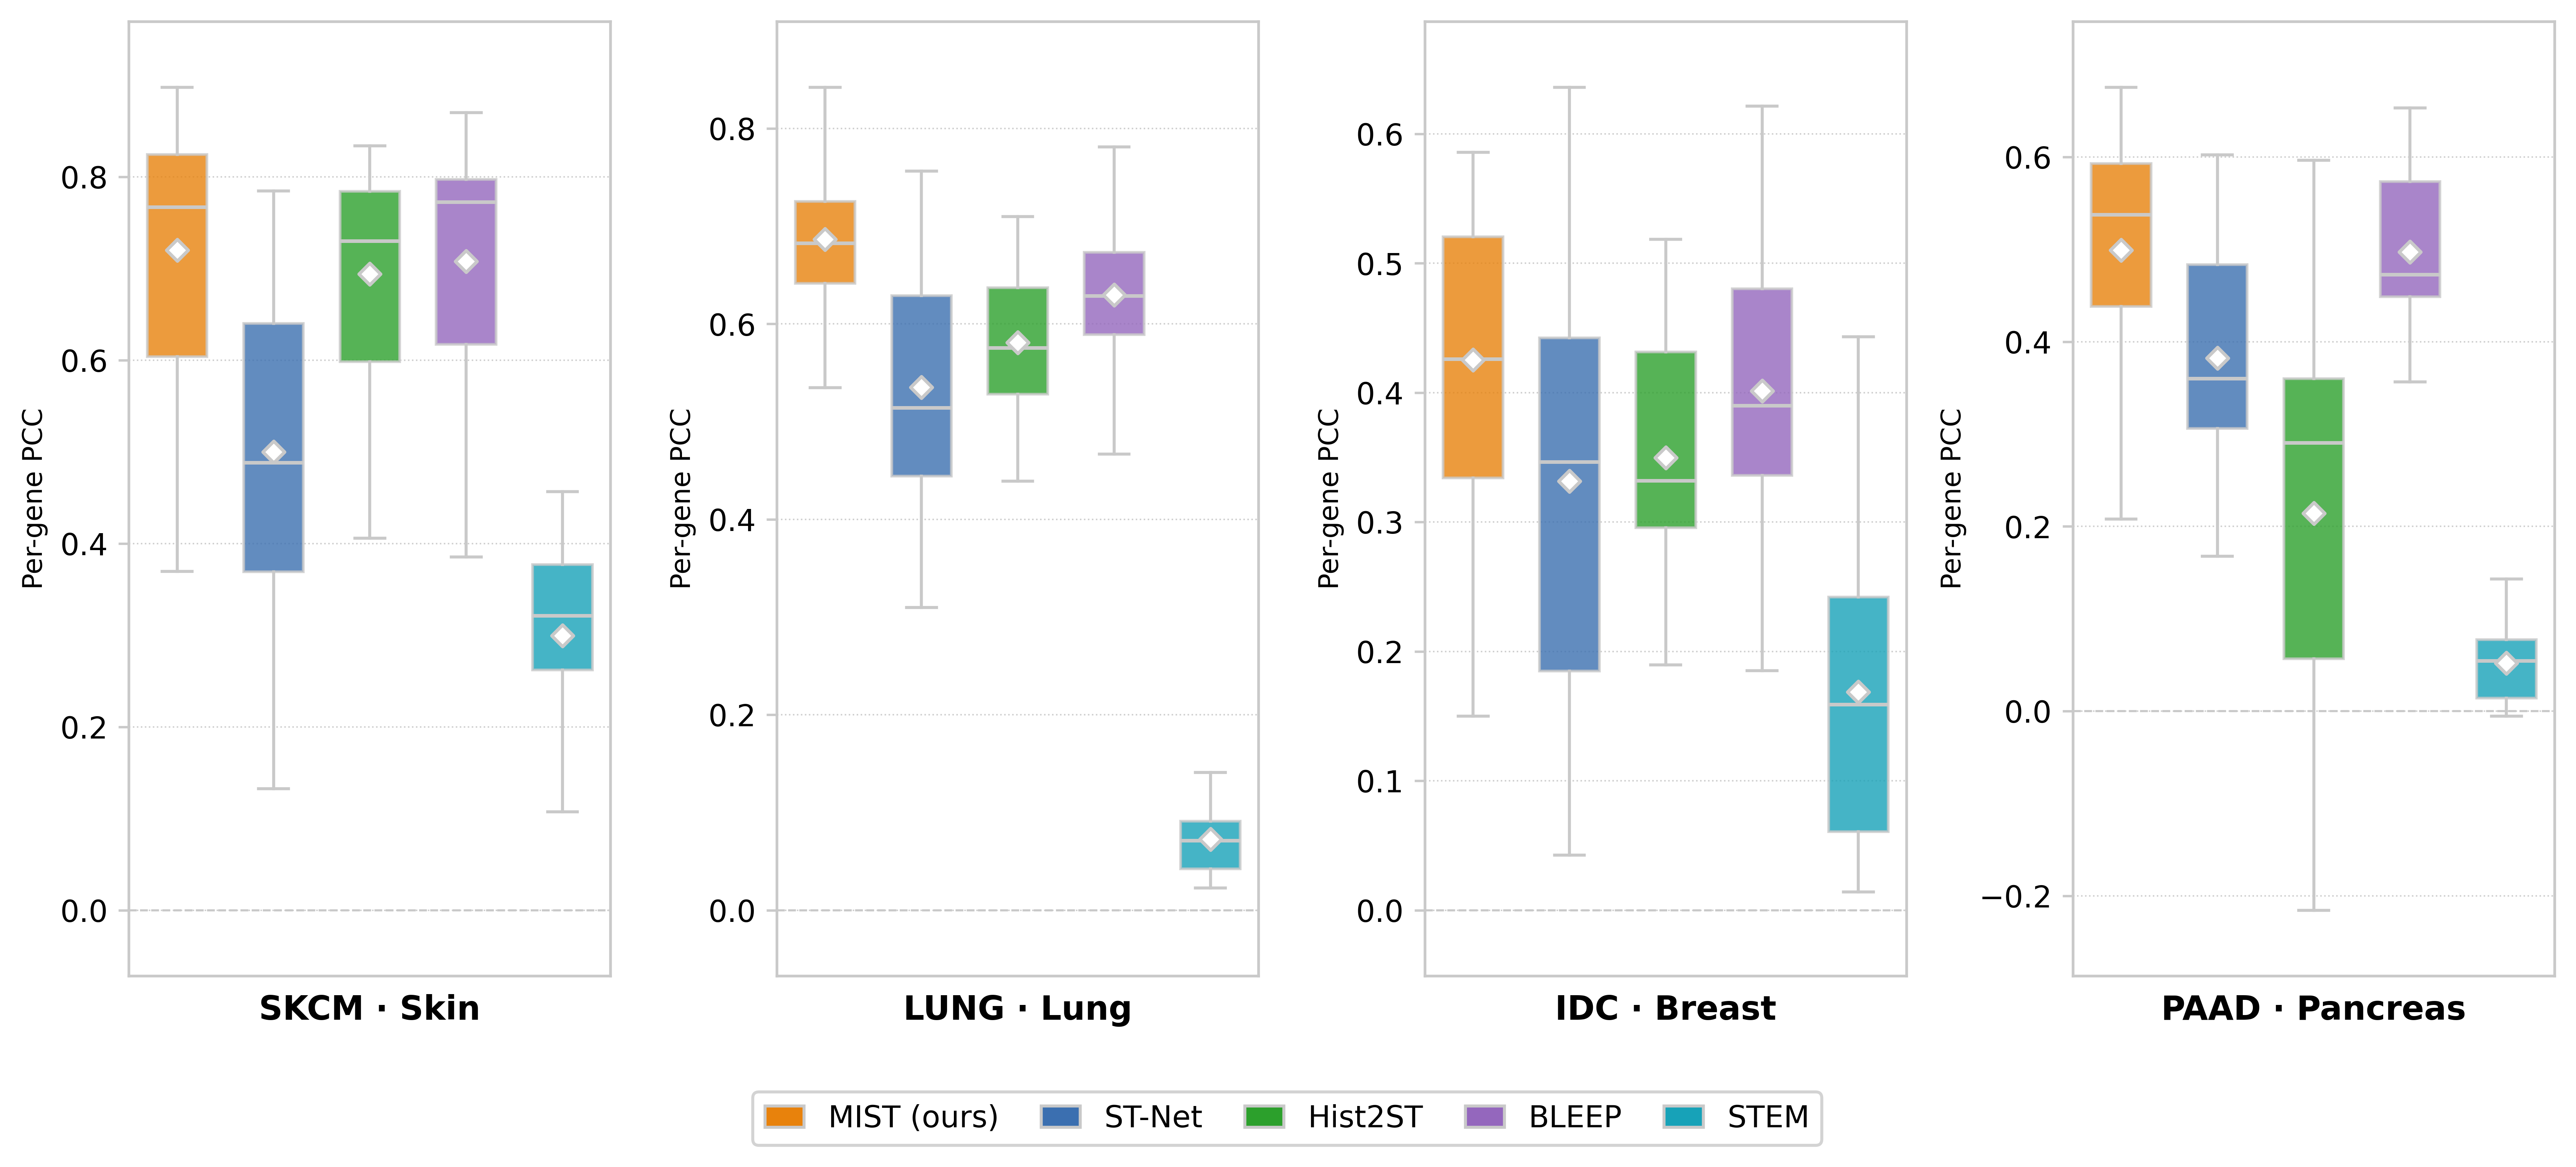
\includegraphics[width=\linewidth]{figures/box_looo6_4panel.png}
\caption{\textbf{Per-cohort cross-organ LOOO accuracy} (four representative held-out cohorts; kidney
and prostate omitted for readability, frozen UNI+CONCH). One panel per held-out cohort; box = per-gene
PCC over three seeds, $\Diamond$ = mean. \morph{} (orange) leads in all four panels, and wins all six
held-out organs in the complete table (Appendix~\ref{app:looo_complete}, Table~\ref{tab:looo_6organ}).}
\label{fig:box_looo5}
\end{figure}

\FloatBarrier
\medskip
\subsection{RQ3: What drives accuracy and coordinate invariance?}
\label{sec:design}
Given \morph{}'s accuracy, we next ask \emph{which} components drive it and whether its coordinate
invariance holds in practice. To isolate each context stream, we run a factorial study over all eight
combinations of local (L), global (G), and slide-level (S) context on the six-organ pooled set
(Table~\ref{tab:ablation}). The full model (L\,+\,G\,+\,S) is best (PCC $0.61$), and among the single
streams local attention is the strongest ($0.60$, versus $0.59$ for global and $0.58$ for slide).
Crucially, replacing the spatial $k$NN neighbors with random ones lowers accuracy ($0.61\!\to\!0.58$
for the full model and $0.60\!\to\!0.58$ for global\,+\,local), showing that the benefit comes from
\emph{spatial} locality rather than added attention alone. This identifies local spatial-neighborhood
aggregation as the primary contributor, which supports the design rationale in RQ3.



Beyond accuracy, we also verify the model's coordinate invariance empirically. As
Table~\ref{tab:invariance} shows, prediction differences under translation and rotation remain below
$6\times10^{-5}$, attributable to floating-point evaluation, and reflection is exact. This numerically
confirms the analytic guarantee, completing the answer to RQ3.

\begin{keybox}
\textbf{Key Finding (RQ3):} Local spatial-neighborhood attention is the primary driver of accuracy
(the full L\,+\,G\,+\,S model scores $0.61$, local is the strongest single stream, and spatial $k$NN
neighbors beat random ones), and the predictor is provably invariant to spot translation, rotation,
and reflection.
\end{keybox}

\begin{table}[H]
\centering
\caption{\textbf{Context-stream ablation (six-organ POOLED, no COAD).} Each row toggles a subset of
\morph{}'s local (L), global (G), and slide (S) context streams on the six-organ POOLED set
(CCRCC/IDC/LUNG/PAAD/PRAD/SKCM; frozen UNI+CONCH, 14-gene, 5-fold). POOLED PCC$\uparrow$, MSE$\downarrow$,
and MAE$\downarrow$ are mean$_{\text{std}}$ over three seeds; best per column in \best{bold}. The last
row replaces spatial-kNN local attention with random neighbours. The complete model (L+G+S) is best on
PCC and MSE; local attention is the dominant stream.}
\label{tab:ablation}
\small
\setlength{\tabcolsep}{5pt}
\resizebox{\linewidth}{!}{%
\begin{tabular}{ll ccc}
\toprule
Configuration & Streams & PCC $\uparrow$ & MSE $\downarrow$ & MAE $\downarrow$ \\
\midrule
Global\,+\,Local         & L\,+\,G       & $0.60{\pm}0.01$ & $0.46{\pm}0.02$ & $0.41{\pm}0.01$ \\
Global\,+\,Slide         & G\,+\,S       & $0.57{\pm}0.04$ & $0.52{\pm}0.13$ & $0.44{\pm}0.05$ \\
Global only              & G             & $0.59{\pm}0.00$ & $0.47{\pm}0.02$ & $0.42{\pm}0.01$ \\
Local\,+\,Slide          & L\,+\,S       & $0.60{\pm}0.01$ & $0.43{\pm}0.03$ & \best{$0.40{\pm}0.02$} \\
Local only               & L             & $0.60{\pm}0.02$ & $0.46{\pm}0.05$ & $0.41{\pm}0.02$ \\
Slide only               & S             & $0.58{\pm}0.02$ & $0.47{\pm}0.03$ & $0.42{\pm}0.02$ \\
Global\,+\,Local (random nbr.) & L$_{\text{rand}}$\,+\,G & $0.58{\pm}0.01$ & $0.45{\pm}0.01$ & \best{$0.40{\pm}0.00$} \\
Full, random nbr.        & L$_{\text{rand}}$\,+\,G\,+\,S & $0.58{\pm}0.01$ & $0.47{\pm}0.01$ & $0.41{\pm}0.00$ \\
\midrule
\morph{} (ours)          & L\,+\,G\,+\,S & \best{$0.61{\pm}0.01$} & \best{$0.42{\pm}0.01$} & \best{$0.40{\pm}0.01$} \\
\bottomrule
\end{tabular}}
\end{table}

\begin{table}[t]
\centering
\caption{\textbf{Numerical coordinate-invariance check.} Maximum absolute prediction difference when only the spot coordinates are transformed (randomly initialized model, 257-spot synthetic slide).}
\label{tab:invariance}
\small
\begin{tabular}{l r}
\toprule
Transformation & Max.\ abs.\ difference \\
\midrule
Translation & $5.97\times10^{-5}$ \\
Rotation    & $1.97\times10^{-5}$ \\
Reflection  & $0$ \\
Spot permutation & $5.96\times10^{-7}$ \\
\bottomrule
\end{tabular}
\end{table}

\begin{figure*}[t]
\centering
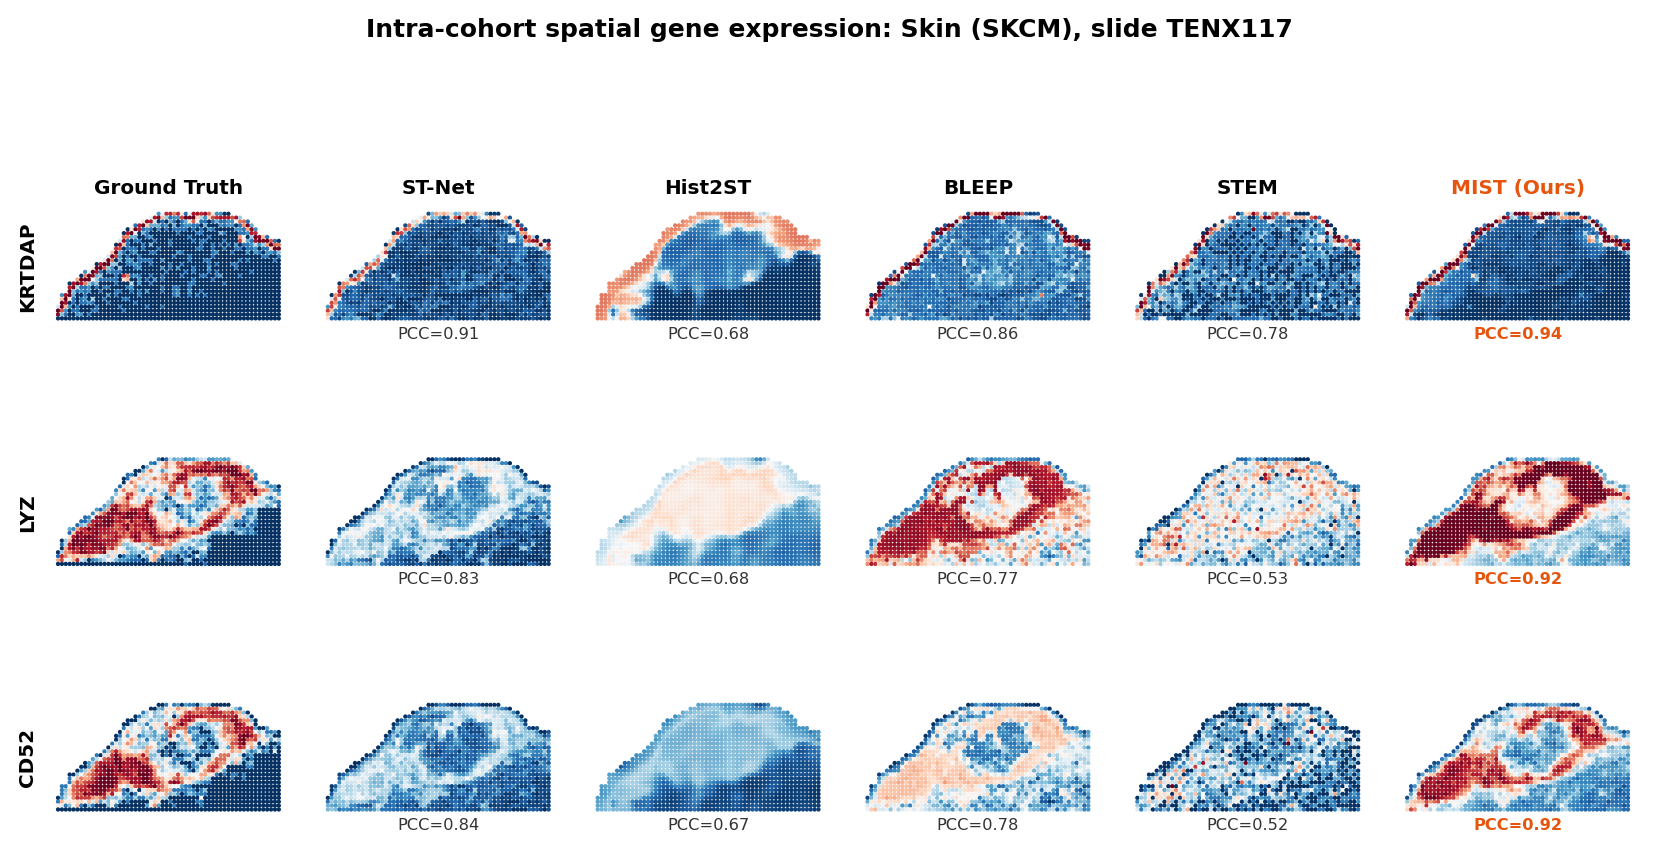
\includegraphics[width=\linewidth]{figures/qualitative_skcm.png}
\caption{\textbf{Qualitative spatial expression maps} for a held-out skin (SKCM) slide (TENX117),
three genes (rows). Each panel colors every spot by expression; \morph{} (right) most faithfully
recovers the ground-truth spatial structure: the perivascular ring for \emph{LYZ}/\emph{CD52} and
the epidermal edge for \emph{KRTDAP}. It attains the highest per-gene PCC (in orange), whereas STEM
is noisy and Hist2ST over-smooths. Predictions use identical frozen UNI+CONCH features.}
\label{fig:qualitative}
\end{figure*}

\FloatBarrier
\medskip





\subsection{RQ4: Spatial structure preservation}
\label{sec:structure}
Accurate per-gene prediction does not by itself guarantee that predictions preserve coherent tissue
regions, so we finally ask whether \morph{} recovers spatial \emph{structure}. To test this, we cluster
spots (KMeans, $k{=}6$ domains) from either predicted or measured expression and compare the induced
partitions using the adjusted Rand index (ARI) and normalized mutual information (NMI) on held-out
slides of the six-organ subset (Table~\ref{tab:downstream5}). \morph{} leads on both ARI ($0.173$) and
NMI ($0.242$), ahead of the strongest baseline on each metric (BLEEP at $0.147$ ARI, ST-Net at $0.201$
NMI). Absolute scores vary widely across slides (std $\approx$ mean), so the cohort means alone are hard
to interpret; a \emph{paired per-slide} comparison, however, is decisive (Figure~\ref{fig:spatial_scatter}): \morph{}
beats BLEEP on $78\%$ of slides for ARI and $90\%$ for NMI ($n{=}58$ held-out slides; Wilcoxon
$p<0.001$ for both).
\morph{} therefore recovers spatial domains more faithfully than the strongest baseline, even though the
absolute agreement remains modest; the full seven-cohort version appears in Appendix~\ref{app:spatial}.

\begin{table}[h]
\centering
\caption{\textbf{Spatial-domain recovery (six-organ subset).} ARI/NMI between domains clustered
(KMeans, $k{=}6$) from predicted vs.\ measured expression on held-out slides of CCRCC, IDC, LUNG,
PAAD, PRAD, and SKCM (COAD excluded); mean$_{\mathrm{std}}$ over three seeds, higher is better,
best per column in \best{bold}.}
\label{tab:downstream5}
\small
\setlength{\tabcolsep}{6pt}
\begin{tabular}{l cc}
\toprule
Method & ARI $\uparrow$ & NMI $\uparrow$ \\
\midrule
ST-Net~\cite{he2020stnet}      & $0.140_{0.11}$ & $0.201_{0.12}$ \\
Hist2ST~\cite{zeng2022hist2st} & $0.133_{0.11}$ & $0.180_{0.11}$ \\
BLEEP~\cite{xie2023bleep}      & $0.147_{0.12}$ & $0.197_{0.13}$ \\
STEM~\cite{zhu2025diffusion}   & $0.101_{0.12}$ & $0.136_{0.14}$ \\
\midrule
\morph{}                       & \best{$0.173_{0.14}$} & \best{$0.242_{0.14}$} \\
\bottomrule
\end{tabular}
\end{table}

\begin{figure}[H]
\centering
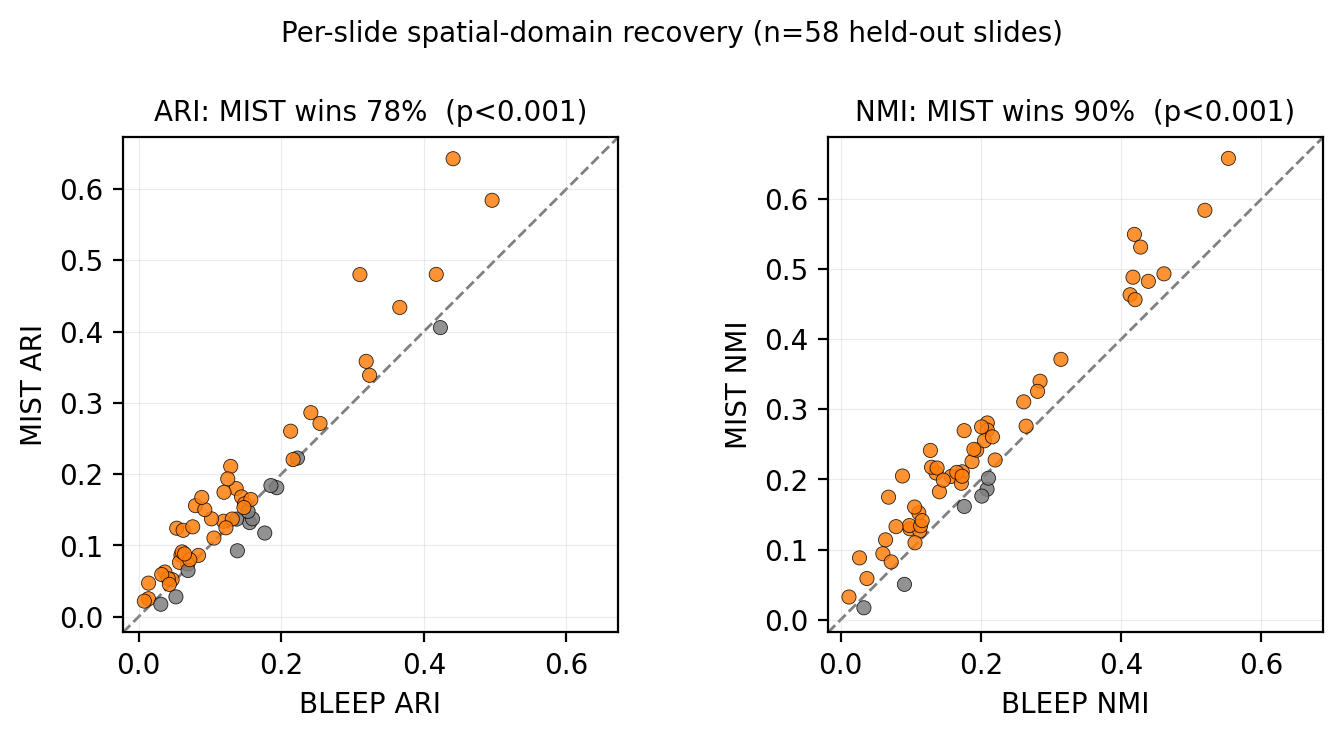
\includegraphics[width=0.9\linewidth]{figures/spatial_ari_nmi.png}
\caption{\textbf{Per-slide spatial-domain recovery}, \morph{} (\emph{y}) vs.\ BLEEP (\emph{x}) on the
$n{=}58$ held-out slides. Each point is one slide; orange marks slides where \morph{} wins; the dashed
line is $y{=}x$. Points spread widely (large across-slide variance) yet lie mostly above the diagonal,
so \morph{} improves ARI on $78\%$ and NMI on $90\%$ of slides (Wilcoxon $p<0.001$ for both).}
\label{fig:spatial_scatter}
\end{figure}

\begin{keybox}
\textbf{Key Finding (RQ4):} \morph{} reconstructs spatial domains more faithfully than the strongest
baseline: paired per slide, it improves both ARI and NMI on $78$--$90\%$ of held-out slides
($n{=}58$; Wilcoxon $p<0.001$; Figure~\ref{fig:spatial_scatter}), though the absolute domain agreement
remains modest.
\end{keybox}

\FloatBarrier
\medskip
\subsection{RQ5: Computational efficiency}
\label{sec:efficiency}
Finally, we ask whether this accuracy comes at a practical cost. \morph{} contains $4.88$M parameters
and predicts a complete slide in a single forward pass (Appendix~Table~\ref{tab:complexity}). Its
advantage is not the smallest footprint: ST-Net and BLEEP have fewer parameters, but \morph{} instead
pairs multi-scale spatial context with direct, non-iterative inference. Concretely, model-only latency
grows from $3.5$\,ms for 500 spots to $64.7$\,ms for 10,000 spots on an A100, with $3.1$\,GiB peak
allocated memory at the largest size (Appendix~Table~\ref{tab:scaling}; feature extraction and disk I/O
excluded). In contrast, STEM's iterative diffusion is the only approach with substantially higher
latency. \morph{} therefore answers RQ5 by delivering its accuracy at single-pass inference cost.

\begin{keybox}
\textbf{Key Finding (RQ5):} \morph{} predicts a whole slide in one forward pass ($4.88$M parameters;
$64.7$\,ms and $3.1$\,GiB for 10,000 spots on an A100), pairing its accuracy with efficient,
non-iterative inference, unlike the diffusion baseline.
\end{keybox}





\FloatBarrier
Three findings merit emphasis. First, a compact direct predictor is competitive when features,
gene panels, splits, and model selection are controlled; the $11.6\%$ relative gain over the
strongest baseline rests on matched experimental conditions, not a larger model. Second, pooled
multi-organ performance is not a substitute for unseen-organ evaluation: the drop from $0.760$
(pooled) to $0.490$ (LOOO) shows that anatomical shift remains a separate and harder problem. Third,
local spatial-neighborhood attention is the dominant contributor in the factorial study; global and
slide pathways provide moderate complementary gains, and the complete model (L\,+\,G\,+\,S) achieves
the best mean on the pooled evaluation.

Direct and generative models serve different purposes. STEM \cite{zhu2025diffusion} models a
conditional expression distribution and can represent one-to-many uncertainty through iterative
sampling. \morph{} produces a point estimate optimized for correlation and squared error. Its
benefits, including deterministic, single-pass inference and explicit coordinate invariance, do not
imply that morphology uniquely determines expression.

\textbf{Limitations.} The evaluation predicts $50$ genes from frozen UNI+CONCH embeddings; results
may not extend to transcriptome-scale output or end-to-end image encoding. LOOO uses a fixed
benchmark panel and does not test platform or institution shift simultaneously. Coordinate invariance
holds only for the spatial pathway with fixed image features; rotating the histology image can change
its frozen embedding. Domain-recovery analysis covers only two baselines and has high slide-level
variance. Pooled folds are sample-disjoint but cannot be verified as patient-disjoint where patient
identifiers are unavailable.

\section{Conclusion and Future Work}
We developed \morph{}, a coordinate-invariant local--global spatial transformer for predicting gene
expression from histology. Pairwise-distance encoding makes the spatial pathway invariant to rigid
coordinate transformations by construction, while three parallel context signals: local $k$NN
attention, global self-attention, and slide-level pooling, together produce complete-slide
predictions in a single pass. These design choices directly address our design goals that
multi-scale context is necessary and that architectural positional bias should not break under
coordinate shift. Under matched HEST-1k evaluation, \morph{} improves mean intra-cohort correlation
and remains competitive in LOOO transfer; the pooled-to-LOOO gap exposes the remaining difficulty of
anatomical transfer as the central open challenge.

For future work, it would be valuable to explore how conditioning on slide-level metadata (organ
type, sequencing platform) can narrow this anatomical gap, for instance, through FiLM or
adaptive layer normalisation conditioners that are available at inference time without requiring
expression labels. Scaling the gene panel beyond 50 genes, incorporating end-to-end image encoding,
and combining \morph{}'s geometric structure with calibrated generative uncertainty modeling
(as in STEM) are further natural directions.

\subsection*{AI use statement}
Generative AI tools assisted with manuscript organization, language editing, ICLR formatting, and
consistency checks between narrative claims and reported tables. They were not used to generate
experimental data or execute model experiments. The authors reviewed all AI-assisted revisions and
take responsibility for the final content of this work.

\bibliographystyle{iclr2027_conference}
\bibliography{references}

\clearpage
\appendix
\etocdepthtag.toc{supp}
\clearpage
\begin{center}
{\LARGE\scshape Supplementary Material}\\[1.2em]
{\large\scshape Table of Contents}
\end{center}
\vspace{0.8em}
\etocsettagdepth{mainbody}{none}
\etocsettagdepth{supp}{subsection}
\etocsettocstyle{}{}
\tableofcontents
\clearpage

\section{Dataset}
\label{app:cohort_stats}

Table~\ref{tab:cohort_stats} lists the number of samples, total spots, and cross-validation folds
for each HEST-1k cohort.
Two organ groups in HEST-1k contain multiple cohorts: breast (IDC + LYMPH\_IDC) and
colorectal (COAD + READ).
Within each group the constituent cohorts differ substantially in size: IDC has $2.25\times$ more
spots than LYMPH\_IDC (44{,}974 vs.\ 19{,}964), and COAD has $2.2\times$ more spots than READ
(18{,}523 vs.\ 8{,}407).
To avoid misrepresentation from unweighted averaging over unequal cohorts, Table~\ref{tab:main}
uses \textbf{IDC} as the representative breast cohort and \textbf{COAD} as the representative
colorectal cohort, discarding the smaller partner cohorts (LYMPH\_IDC and READ) from the
organ-level rows. This choice maximises statistical reliability of each organ-level estimate.
Our cross-organ experiments (leave-one-organ-out and pooled) use the \textbf{six} cohorts marked in
Table~\ref{tab:cohort_stats}: CCRCC (kidney, 24 samples / 74{,}220 spots), IDC (breast, 4 / 44{,}974),
LUNG (lung, 2 / 7{,}505), PAAD (pancreas, 3 / 9{,}793), PRAD (prostate, 23 / 62{,}710), and SKCM
(skin, 2 / 5{,}716); COAD, READ, LYMPH\_IDC, and HCC are not used in the cross-organ setting.

\begin{table}[H]
\centering
\caption{\textbf{HEST-1k cohort statistics.} Spots counted after barcode filtering. Folds = number
of train/test splits in the per-cohort cross-validation. The six cohorts marked \checkmark
(CCRCC, IDC, LUNG, PAAD, PRAD, SKCM) form the no-COAD cross-organ evaluation set used in our
leave-one-organ-out and pooled experiments; LYMPH\_IDC, COAD, READ, and HCC (liver) are not used
there (HCC has a near-zero signal floor).}
\label{tab:cohort_stats}
\small
\begin{tabular}{l l r r r c}
\toprule
Cohort & Organ & Samples & Spots & Folds & 6-organ set \\
\midrule
IDC          & Breast      & 4 & 44{,}974 & 4 & \checkmark \\
LYMPH\_IDC   & Breast      & 4 & 19{,}964 & 4 &            \\
COAD         & Colorectal  & 4 & 18{,}523 & 2 &            \\
READ         & Colorectal  & 4 &  8{,}407 & 2 &            \\
CCRCC        & Kidney      & 24 & 74{,}220 & 6 & \checkmark \\
HCC          & Liver$^*$   &  2 &  4{,}248 & 2 &            \\
LUNG         & Lung        &  2 &  7{,}505 & 2 & \checkmark \\
PAAD         & Pancreas    &  3 &  9{,}793 & 3 & \checkmark \\
PRAD         & Prostate    & 23 & 62{,}710 & 2 & \checkmark \\
SKCM         & Skin        &  2 &  5{,}716 & 2 & \checkmark \\
\bottomrule
\end{tabular}
\begin{minipage}{\linewidth}
\vspace{2pt}
\footnotesize $^*$HCC (liver) is included here for completeness but excluded from
Table~\ref{tab:main}; all baselines score near zero on this cohort due to low spatial
gene-expression variance.
\end{minipage}
\end{table}

\paragraph{Split granularity and patient disjointness.}
Each ``sample'' in Table~\ref{tab:cohort_stats} is a distinct HEST-1k slide (a whole-slide section),
and every fold is \emph{slide-disjoint}: no slide is shared between training and test, the pooled
regime holds out entire slides, and the leave-one-organ-out regime holds out entire organs. HEST-1k
patient/donor identifiers are not distributed with the per-slide data in our pipeline, so for a cohort
in which one donor may contribute several slides we cannot verify patient-level disjointness. The
intra-cohort and pooled numbers should therefore be read as \emph{slide-level} generalization and
could be optimistic if a cohort mixes multiple slides from the same patient; this risk is largest for
the two multi-slide cohorts, CCRCC (24 slides) and PRAD (23 slides), and small for the remaining
cohorts (IDC~4, PAAD~3, LUNG~2, SKCM~2 slides). Importantly, the cross-organ LOOO transfer results
(our central generalization claim) are unaffected, because an entire organ (and hence a disjoint set
of patients) is withheld at test time.

\section{Extended Related Work}
\label{app:related}

\paragraph{Machine-learning prediction of gene expression from histology.}
ST-Net~\cite{he2020stnet} established patch-level regression. Hist2ST~\cite{zeng2022hist2st} adds
spatial context through a graph over neighboring spots, while BLEEP~\cite{xie2023bleep} aligns image
and expression embeddings for cross-modal retrieval. STEM~\cite{zhu2025diffusion} instead treats
expression prediction as conditional generation. These methods use different features, gene panels,
splits, and selection procedures, so their published scores do not isolate architectural gains; our
comparisons therefore use a matched protocol. \morph{} is a deterministic point predictor and does
not model the full conditional expression distribution.

\paragraph{Geometric structure and coordinate invariance.}
Spatial prediction depends on the coordinate representation supplied to a model. Absolute position
embeddings can encode location within a particular coordinate frame, but their output may change when
an equivalent tissue layout is translated, rotated, or reflected. Geometric networks address this by
constructing interactions from relative quantities~\cite{satorras2021egnn}. \morph{} uses pairwise
Euclidean distances, which are preserved by translations, rotations, and reflections; the guarantee
applies to the spatial pathway for fixed histology features, not to rotations of the image-encoder
input.

\paragraph{Generalization across samples and organs.}
HEST-1k~\cite{jaume2024hest} spans many cohorts and organs. Within-cohort evaluation can exploit
organ-specific morphology or acquisition effects. We therefore distinguish pooled cross-validation,
which holds out samples while retaining their organ types in training, from LOOO, which withholds an
entire organ and provides a stricter test of anatomical transfer.

\paragraph{Positioning of \morph{}.}
\morph{} connects these three directions: an inductive-bias-explicit spatial transformer for direct
regression, evaluated under a matched cross-cohort protocol. Unlike absolute position encodings or
frame-averaging strategies, its coordinate pathway is invariant by construction. Unlike generative
models, it does not represent expression uncertainty; its advantage is deterministic, single-pass
inference with explicit geometric structure. Unlike prior evaluations that report within-cohort
accuracy only, our controlled comparison separates interpolation from anatomical transfer, making the
difficulty of organ shift directly measurable.

\section{Extended Experimental Setup}
\label{app:extended_setup}

\paragraph{Dataset and preprocessing.}
We evaluate on HEST-1k \cite{jaume2024hest} using the cohorts of Table~\ref{tab:cohort_stats}; HCC,
LYMPH\_IDC, and READ are excluded under the documented quality and split criteria, and the six
cohorts marked in that table (CCRCC, IDC, LUNG, PAAD, PRAD, SKCM) form the cross-organ set. We use the
provided patient-stratified folds, $\log(1+x)$ normalization, and frozen UNI+CONCH features (1536-d).
Unless stated otherwise, targets are the 50-gene HEST HVG panel. The panel study additionally uses
matched 50-gene DEG (Wilcoxon selection across Leiden clusters) and HMHVG (mean-and-variability
selection after variance filtering) panels (Table~\ref{tab:panel_strategy}).

\paragraph{Evaluation protocol.}
Intra-cohort training fits a model within each cohort. Pooled five-fold validation trains across
organs while holding out slide-level samples; organ identity defines the protocol but is not a model
input. LOOO trains on all-but-one organ and tests the held-out organ. We report PCC, SCC, and MSE
averaged over outer folds and three seeds. Checkpoints are selected on inner validation and evaluated
once on the outer test fold; single-slide folds use disjoint spots for inner validation. Patient-level
disjointness is not guaranteed where identifiers are unavailable.

\paragraph{Baselines and implementation.}
We compare with ST-Net \cite{he2020stnet}, Hist2ST \cite{zeng2022hist2st}, BLEEP \cite{xie2023bleep},
and STEM \cite{zhu2025diffusion} under matched features, panels, splits, budgets, and checkpoint
selection.
\morph{} uses four layers, width 256, four heads, eight neighbors, 16 radial bases, and 4.88M
parameters. AdamW training uses learning rate $10^{-3}$, weight decay $10^{-2}$, cosine decay,
gradient clipping, 100 epochs maximum, patience 20, and at most 3,000 spots per step.

\section{Encoder Ablation}
\label{app:encoder}
We repeat the intra-cohort PCC@50 comparison (the 50-gene block of Table~\ref{tab:main}, which uses the concatenated UNI\,+\,CONCH features) with each foundation encoder \emph{in isolation}: UNI only (ViT-L/16, 1024-d) and CONCH only (512-d), holding models, cohorts, gene panels, splits, and training budget fixed (Table~\ref{tab:encoder}). \morph{} remains the most accurate encoder-averaged method under both UNI-only and CONCH-only features.

\begin{table}[H]
\centering
\caption{\textbf{Encoder ablation: intra-cohort PCC@50 with each foundation encoder in isolation.} UNI only (1024-d) vs.\ CONCH only (512-d), per cohort; mean$_{\text{std}}$ over three seeds; best per row in \best{bold}. Compare with the UNI\,+\,CONCH (1536-d) results in Table~\ref{tab:main}.}
\label{tab:encoder}
\setlength{\tabcolsep}{3pt}\renewcommand{\arraystretch}{1.05}
\resizebox{\linewidth}{!}{%
\begin{tabular}{ll ccccc}
\toprule
Encoder & Cohort & ST-Net & Hist2ST & BLEEP & STEM & \morph{} (Ours) \\
\midrule
\multirow{7}{*}{\rotatebox[origin=c]{90}{\textbf{\shortstack{UNI\\(1024-d)}}}} & IDC~\tiny{Breast} & $0.538{\pm}0.008$ & $0.250{\pm}0.067$ & $0.508{\pm}0.005$ & $0.436{\pm}0.005$ & \best{$0.569{\pm}0.009$} \\
 & CCRCC~\tiny{Kidney} & $0.172{\pm}0.010$ & $0.214{\pm}0.015$ & $0.184{\pm}0.007$ & $0.116{\pm}0.002$ & \best{$0.264{\pm}0.010$} \\
 & LUNG~\tiny{Lung} & $0.482{\pm}0.012$ & $0.378{\pm}0.097$ & $0.559{\pm}0.007$ & $0.393{\pm}0.009$ & \best{$0.590{\pm}0.005$} \\
 & PAAD~\tiny{Pancreas} & $0.353{\pm}0.022$ & $0.243{\pm}0.061$ & \best{$0.393{\pm}0.035$} & $0.227{\pm}0.017$ & $0.392{\pm}0.040$ \\
 & PRAD~\tiny{Prostate} & $0.251{\pm}0.008$ & $0.322{\pm}0.020$ & $0.343{\pm}0.009$ & $0.190{\pm}0.010$ & \best{$0.394{\pm}0.003$} \\
 & SKCM~\tiny{Skin} & $0.632{\pm}0.010$ & $0.510{\pm}0.015$ & $0.639{\pm}0.015$ & $0.471{\pm}0.031$ & \best{$0.694{\pm}0.001$} \\
\cmidrule(lr){2-7}
 & \textbf{Average} & $0.405$ & $0.319$ & $0.438$ & $0.305$ & \best{$0.484$} \\
\midrule
\multirow{7}{*}{\rotatebox[origin=c]{90}{\textbf{\shortstack{CONCH\\(512-d)}}}} & IDC~\tiny{Breast} & $0.515{\pm}0.007$ & $0.264{\pm}0.018$ & $0.496{\pm}0.011$ & $0.396{\pm}0.011$ & \best{$0.551{\pm}0.004$} \\
 & CCRCC~\tiny{Kidney} & $0.160{\pm}0.010$ & $0.126{\pm}0.026$ & $0.141{\pm}0.012$ & $0.078{\pm}0.001$ & \best{$0.222{\pm}0.010$} \\
 & LUNG~\tiny{Lung} & $0.517{\pm}0.001$ & $0.435{\pm}0.006$ & \best{$0.576{\pm}0.003$} & $0.386{\pm}0.030$ & $0.554{\pm}0.005$ \\
 & PAAD~\tiny{Pancreas} & $0.372{\pm}0.035$ & $0.186{\pm}0.035$ & $0.384{\pm}0.033$ & $0.251{\pm}0.028$ & \best{$0.387{\pm}0.045$} \\
 & PRAD~\tiny{Prostate} & $0.327{\pm}0.003$ & $0.322{\pm}0.009$ & $0.364{\pm}0.010$ & $0.210{\pm}0.013$ & \best{$0.406{\pm}0.006$} \\
 & SKCM~\tiny{Skin} & $0.633{\pm}0.002$ & $0.388{\pm}0.022$ & $0.633{\pm}0.005$ & $0.453{\pm}0.014$ & \best{$0.658{\pm}0.007$} \\
\cmidrule(lr){2-7}
 & \textbf{Average} & $0.421$ & $0.287$ & $0.432$ & $0.296$ & \best{$0.463$} \\
\bottomrule
\end{tabular}%
}
\end{table}

\section{Complete LOOO (Leave-One-Organ-Out) Results}
\label{app:looo_complete}
Table~\ref{tab:looo_6organ} reports the complete per-cohort leave-one-organ-out transfer results on
the six-organ subset summarised in the main text (Section~\ref{sec:transfer}, Figure~\ref{fig:box_looo5}).
Each fold holds out one entire organ and trains on the other five, using leakage-safe per-fold gene
panels and identical frozen UNI\,+\,CONCH features. \morph{} wins every held-out cohort and the
average ($0.422$).

\begin{table}[H]
\centering
\caption{\textbf{Cross-organ LOOO transfer on a six-organ subset} (kidney, breast, lung, pancreas,
prostate, skin; COAD excluded), per-cohort Pearson $\uparrow$. Self-contained leave-one-organ-out:
each fold holds out one organ and trains on the other five, with leakage-safe per-fold gene panels.
Identical frozen UNI\,+\,CONCH features (1536-dim); mean$_{\text{std}}$ over three seeds; best per row
in \best{bold}. \morph{} wins every cohort and the average.}
\label{tab:looo_6organ}
\setlength{\tabcolsep}{3pt}
\resizebox{\linewidth}{!}{%
\begin{tabular}{l cc cc c}
\toprule
Cohort & ST-Net~\tiny{NBE'20} & Hist2ST~\tiny{BIB'22} & BLEEP~\tiny{NeurIPS'23} & STEM~\tiny{ICLR'25}$^\dagger$ & \morph{} (Ours) \\
\midrule
CCRCC~\tiny{Kidney}    & $0.074{\pm}0.00$ & $0.064{\pm}0.01$ & $0.058{\pm}0.00$ & $0.024{\pm}0.01$ & \best{$0.098{\pm}0.01$} \\
IDC~\tiny{Breast}      & $0.332{\pm}0.02$ & $0.350{\pm}0.00$ & $0.401{\pm}0.04$ & $0.131{\pm}0.08$ & \best{$0.425{\pm}0.03$} \\
LUNG~\tiny{Lung}       & $0.535{\pm}0.07$ & $0.581{\pm}0.00$ & $0.630{\pm}0.00$ & $0.067{\pm}0.00$ & \best{$0.687{\pm}0.02$} \\
PAAD~\tiny{Pancreas}   & $0.382{\pm}0.00$ & $0.214{\pm}0.17$ & $0.497{\pm}0.03$ & $0.052{\pm}0.00$ & \best{$0.499{\pm}0.03$} \\
PRAD~\tiny{Prostate}   & $0.078{\pm}0.01$ & $0.062{\pm}0.01$ & $0.091{\pm}0.00$ & $0.016{\pm}0.00$ & \best{$0.105{\pm}0.01$} \\
SKCM~\tiny{Skin}       & $0.500{\pm}0.09$ & $0.694{\pm}0.02$ & $0.708{\pm}0.01$ & $0.299{\pm}0.00$ & \best{$0.720{\pm}0.03$} \\
\midrule
\textbf{Average}       & $0.317$ & $0.328$ & $0.398$ & $0.098$ & \best{$0.422$} \\
\bottomrule
\end{tabular}%
}\\[2pt]
{\footnotesize $^\dagger$STEM incomplete (1--2 of 3 seeds); values provisional.}
\end{table}

\section{Computation Resources, Model Complexity, and Inference Scaling}
\label{app:compute}
All experiments ran on a shared GPU cluster. Feature extraction and training used NVIDIA GPUs with
compute capability $\geq$~sm\_80 (A100 80GB, A100-PCIe, L40s, and H200); Volta (V100) GPUs are
incompatible with our CUDA-13 / PyTorch build and were excluded.
\begin{itemize}[nosep,leftmargin=1.4em]
\item \textbf{Encoders:} frozen UNI (ViT-L/16, 1024-d) and CONCH (512-d) patch features, concatenated
to 1536-d; no encoder fine-tuning.
\item \textbf{Model:} \morph{} has 4.88M trainable parameters (Table~\ref{tab:complexity}) and predicts
a whole slide in a single forward pass, with no iterative sampling.
\item \textbf{Training:} AdamW with a cosine schedule, 100 epochs with early stopping (patience~20),
nested validation, and a correlation-aware objective; three seeds per configuration.
\item \textbf{Inference:} single-pass; median model-only latency and peak memory versus slide size are
reported in Table~\ref{tab:scaling}, with feature extraction and disk I/O excluded.
\end{itemize}


\begin{table}[H]
\centering
\caption{\textbf{Model complexity.} Parameter counts and inference mechanisms.}
\label{tab:complexity}
\small
\setlength{\tabcolsep}{5pt}
\begin{tabular}{l r l}
\toprule
Model & \#Params (M) & Inference \\
\midrule
ST-Net~\cite{he2020stnet} (NBE'20)      & 0.47  & single-pass \\
Hist2ST~\cite{zeng2022hist2st} (BIB'22) & 2.18  & single-pass \\
BLEEP~\cite{xie2023bleep} (NeurIPS'23)  & 0.54  & single-pass \\
STEM~\cite{zhu2025diffusion} (ICLR'25)    & 34.16 & iterative \\
\midrule
\morph{} (V3) & 4.88 & single-pass \\
\bottomrule
\end{tabular}
\end{table}

\begin{table}[H]
\centering
\caption{\textbf{\morph{} inference scaling on an NVIDIA A100 80GB.} Median model-only latency and
peak allocated GPU memory over synthetic slides; feature extraction and disk I/O are excluded.}
\label{tab:scaling}
\small
\begin{tabular}{r rr}
\toprule
Spots & Latency (ms) & Memory (MiB) \\
\midrule
500    & 3.48  & 43 \\
1,000  & 3.63  & 67 \\
3,000  & 9.36  & 335 \\
5,000  & 21.31 & 842 \\
10,000 & 64.74 & 3,183 \\
\bottomrule
\end{tabular}
\end{table}

\section{Mouse cross-organ diagnostic}
\label{app:mouse}
We evaluate 59 mouse Visium slides spanning seven organs with mouse-specific 50-gene panels. Pooled
performance reaches $0.887$, whereas every method remains near the floor under LOOO; we therefore do
not interpret the latter as evidence of successful cross-species organ transfer.

\begin{table}[H]
\centering
\caption{\textbf{Cross-organ generalization on mouse HEST} (three seeds, mean$_{\text{std}}$).
\textsc{looo}: leave-one-organ-out transfer; \textsc{pooled}: five-fold pooled cross-validation.
PCC$\uparrow$ on 50 mouse HVGs.}
\label{tab:mouse}
\small
\setlength{\tabcolsep}{5pt}
\begin{tabular}{l c c}
\toprule
Method & \textsc{looo} PCC$^\dag$ & \textsc{pooled} PCC \\
\midrule
ST-Net~\cite{he2020stnet}          & $0.013_{0.011}$ & $0.357_{0.036}$ \\
Hist2ST~\cite{zeng2022hist2st}     & $0.018_{0.007}$ & $0.829_{0.028}$ \\
BLEEP~\cite{xie2023bleep}          & $-0.006_{0.003}$ & $0.848_{0.012}$ \\
STEM~\cite{zhu2025diffusion}       & -- & $0.279_{0.009}$ \\
\midrule
\morph{} & \best{$0.018_{0.006}$} & \best{$0.887_{0.005}$} \\
\bottomrule
\end{tabular}
\begin{minipage}{\linewidth}\vspace{2pt}
\scriptsize $^\dag$All \textsc{looo} values are near the floor because the organ-specific gene
panels do not transfer reliably.
\end{minipage}
\end{table}

\section{Spatial-domain recovery}
\label{app:spatial}
\begin{table}[H]
\centering
\caption{\textbf{Spatial-domain recovery (all seven cohorts).} ARI/NMI between domains clustered
(KMeans, $k{=}6$) from predicted vs.\ measured expression on held-out slides of all seven retained
HEST-1k cohorts; mean$_{\mathrm{std}}$ over three seeds, higher is better, best per column in
\best{bold}. Companion to the five-organ Table~\ref{tab:downstream5}.}
\label{tab:downstream}
\small
\setlength{\tabcolsep}{6pt}
\begin{tabular}{l cc}
\toprule
Method & ARI $\uparrow$ & NMI $\uparrow$ \\
\midrule
ST-Net~\cite{he2020stnet}     & $0.149_{0.11}$ & $0.213_{0.13}$ \\
Hist2ST~\cite{zeng2022hist2st} & $0.149_{0.12}$ & $0.197_{0.12}$ \\
BLEEP~\cite{xie2023bleep}      & $0.157_{0.12}$ & $0.209_{0.14}$ \\
STEM~\cite{zhu2025diffusion}   & $0.113_{0.13}$ & $0.152_{0.15}$ \\
\midrule
\morph{}                       & \best{$0.192_{0.15}$} & \best{$0.259_{0.16}$} \\
\bottomrule
\end{tabular}
\end{table}


\section{Statistical Significance}
\label{app:significance}
Table~\ref{tab:significance} reports paired significance tests of \morph{} against BLEEP, the strongest
baseline, in every regime. For intra-cohort and LOOO we pair mean PCC at the (cohort/organ $\times$
seed) level; for pooled at the (fold $\times$ seed) level; and the per-gene row pairs individual
gene PCC (PCC@50) across cohorts. We report the mean difference with a $95\%$ bootstrap confidence
interval, a Wilcoxon signed-rank test, and a paired $t$-test. The intra-cohort advantage is decisive at
every panel size and at the per-gene level ($p<2.5\times10^{-4}$, and $p<10^{-30}$ per gene), and
cross-organ LOOO transfer is also significant ($p<0.02$). The pooled gain is small ($+0.012$) and only
marginally significant (Wilcoxon $p=0.04$, paired $t$ $p=0.06$), consistent with all organs already
being represented in that regime; we therefore treat the pooled result as supportive rather than
decisive.

\begin{table}[H]
\centering
\caption{\textbf{Statistical significance of \morph{} vs.\ BLEEP} (strongest baseline) across regimes.
$\Delta$PCC is the paired mean difference with a $95\%$ bootstrap CI; $p$-values from Wilcoxon
signed-rank and paired $t$-tests. Intra-cohort/LOOO pair at (cohort/organ $\times$ seed); pooled at
(fold $\times$ seed); per-gene at (gene) over PCC@50.}
\label{tab:significance}
\small
\setlength{\tabcolsep}{4pt}
\begin{tabular}{l r cc c c cc}
\toprule
Comparison & $n$ & \morph{} & BLEEP & $\Delta$PCC & 95\% CI & Wilcoxon $p$ & paired-$t$ $p$ \\
\midrule
Intra-cohort, PCC@10  & 18 & $0.600$ & $0.545$ & $+0.056$ & $[0.034,0.077]$ & $2.5{\times}10^{-4}$ & $1.2{\times}10^{-4}$ \\
Intra-cohort, PCC@50  & 18 & $0.496$ & $0.444$ & $+0.051$ & $[0.041,0.062]$ & $7.6{\times}10^{-6}$ & $4.7{\times}10^{-8}$ \\
Intra-cohort, PCC@100 & 18 & $0.559$ & $0.502$ & $+0.057$ & $[0.045,0.070]$ & $7.6{\times}10^{-6}$ & $1.1{\times}10^{-7}$ \\
Per-gene (PCC@50)     & 300 & $0.496$ & $0.444$ & $+0.051$ & --- & $1.7{\times}10^{-38}$ & --- \\
\midrule
Pooled (cross-organ)  & 15 & $0.599$ & $0.587$ & $+0.012$ & $[0.001,0.022]$ & $4.1{\times}10^{-2}$ & $5.6{\times}10^{-2}$ \\
LOOO (cross-organ)    & 18 & $0.422$ & $0.398$ & $+0.025$ & $[0.007,0.041]$ & $1.8{\times}10^{-2}$ & $1.4{\times}10^{-2}$ \\
\bottomrule
\end{tabular}
\end{table}

\section{Proofs of the formal guarantees}
\label{app:formal_guarantees}

\subsection{Proof of Proposition~\ref{prop:coordinate_invariance}}
For every pair of spots $i,j$, orthogonality of $R$ gives
\begin{align}
\left\|R\mathbf{p}_i+\mathbf{t}-(R\mathbf{p}_j+\mathbf{t})\right\|_2
&=\left\|R(\mathbf{p}_i-\mathbf{p}_j)\right\|_2 \\
&=\left\|\mathbf{p}_i-\mathbf{p}_j\right\|_2.
\end{align}
Hence, transforming the coordinate frame leaves the complete distance matrix unchanged. It also
leaves the $k$NN graph, radial basis features, and distance-dependent attention biases unchanged.
The input projection is unchanged because $\mathbf{F}$ is fixed. At every layer, the local pathway
therefore receives the same features, neighbors, and distance biases, while the global and slide
pathways do not use coordinates. Their outputs, the residual fusion, and the feed-forward update are
identical. Induction over the $L$ layers gives identical final representations and predictions,
proving Proposition~\ref{prop:coordinate_invariance}.

\subsection{Proof of Proposition~\ref{prop:permutation_equivariance}}
Let $\mathbf{F}'=Q\mathbf{F}$ and $\mathbf{P}'=Q\mathbf{P}$. The pairwise distance matrix is relabelled
as $\mathbf{D}'=Q\mathbf{D}Q^\top$. Under equivariant tie handling, the $k$NN graph and its radial
basis edge features are relabelled by the same permutation. The input projection and all pointwise
linear maps, layer normalizations, activations, and feed-forward networks commute with $Q$.

For local attention, permuting the spots only relabels each neighborhood and its attention sum, so
the local output is multiplied by $Q$. Global self-attention is likewise permutation equivariant
because its query-key score matrix is transformed by $Q$ on both axes and its value matrix by $Q$.
The slide attention scores are permuted, but their weighted sum is unchanged; broadcasting that same
summary to all spots is equivariant. Consequently, residual fusion preserves equivariance at every
layer. Induction over the layers and application of the pointwise prediction head yield
$f_\theta(Q\mathbf{F},Q\mathbf{P})=Qf_\theta(\mathbf{F},\mathbf{P})$, proving
Proposition~\ref{prop:permutation_equivariance}.


\section{Training Objective Ablation}
\label{app:lossdata}

Table~\ref{tab:lossdata} isolates the contribution of the Pearson correlation term in the
training objective from the architectural design, confirming that the accuracy gap over baselines
is not attributable to the loss function alone.

\begin{table}[H]
\centering
\caption{\textbf{Objective ablation (HEST-1k).} Effect of adding the Pearson correlation term
to the MSE objective; averaged over seven organ groups, three seeds.}
\label{tab:lossdata}
\small
\setlength{\tabcolsep}{6pt}
\begin{tabular}{l l c}
\toprule
Model & Objective & PCC $\uparrow$ \\
\midrule
\morph{} & MSE only    & $0.382$ \\
\morph{} & MSE $+$ PCC & $0.389$ \\
\bottomrule
\end{tabular}
\end{table}

\end{document}
